% !TeX root = ../main.tex

\chapter{Discussion of Results}
\label{ch:discussion}
In this chapter the performance of different food image classification methods is evaluated. In addition the impact of important classifier parameters is compared. 

\section{Hyper Parameter Optimization}
The hyper parameter optimization is done using a simplified grid search and random search. An exhaustive grid search tests every parameter value by using a cartesian product with the other parameters. Due to the high dimensionality of classifier parameters and the high computational cost of classifier training, exhaustive grid search is not possible in a feasible amount of time and Bergstra and Bengio even showed that random search can outperform grid search \cite{Bergstra2012}. Therefore, parameters are tested individually in addition to random searches on important parameters. This is an acceptable tradeoff between accuracy and time since the goal is not to get optimal parameters but to get a general direction of good parameters for this problem. The following section will first focus on the impact of common parameters like SVM kernels or image size on the performance and then attend to more classifier specific parameters like the number of image segments for color histogram features. 

	\subsection{SVMs and K-nearest Neighbors}
	\begin{table}[htb]
		\begin{tabular*}{\columnwidth}{@{\extracolsep{\stretch{1}}}*{6}{c}@{}}
			\toprule
			Model	 & Color & SIFT  & SURF  & ORB	 & LBP \\ \midrule
			Linear	 & 0.418 & 0.444 & 0.407 & 0.285 & 0.312\\
			Poly	 & 0.494 & 0.347 & 0.339 & 0.282 & \underline{0.519} \\
			RBF		 & 0.125 & 0.523 & 0.455 & 0.263 & 0.364\\
			$\chi^2$ & \underline{0.593} & \underline{0.648} & \underline{0.606} & \underline{0.423} & 0.391 \\
			KNN 	 & 0.412 & 0.294 & 0.364 & 0.258 & 0.431  \\ \bottomrule
		\end{tabular*}
		\caption{Results of classifiers with linear SMV kernel, Polynomial SVM kernel, \gls{rbf} SVM kernel, additive $\chi^2$ SVM kernel and \gls{knn}. Best results are underlined. Test details: HI-4, SI-7, SU-7, O-1, LBP-1}
		\label{tab:resultModels}
	\end{table}
	For classifiers, the model that they are trained on, is the most important parameter. Color histograms, SIFT, SURF, ORB and LBP were tested on the k-nearest Neighbors model and SVMs with four different kernels:
	\begin{itemize}
		\item Linear kernel {(OpenCV)}
		\item Polynomial kernel with degree 2 {(OpenCV)}
		\item \gls{rbf} kernel {(OpenCV)}
		\item Additive $\chi^2$ kernel {(sklearn)}
	\end{itemize} 
	The results are shown in table \ref{tab:resultModels}. The classifiers were not trained with optimal parameters so it is not possible to deduct a classifier ranking based on this evaluation.
	
	Not surprisingly, the $\chi^2$ SVM kernel performs best over all feature classifiers {(except LBP)} because in general, $\chi^2$ kernels are best suited for histogram style feature vectors and those classifiers are all histogram classifiers. However, it should be noted that training and predicting a classifier with a $\chi^2$ kernel can take more than 2 times longer than the same process with a polynomial kernel. Interestingly, the results for \gls{knn} were better than expected considering the fact that \gls{knn} is extremely overfitting on this dataset even for a high k. \gls{knn} achieves an accuracy of 0.960 on the training partition and only 0.363 on the test partition for SURF features for example. Even the worst SVM kernel do not overfitt that much.
	
	\subsection{Image Resolution}
	\begin{figure}[htb]
		\centering
		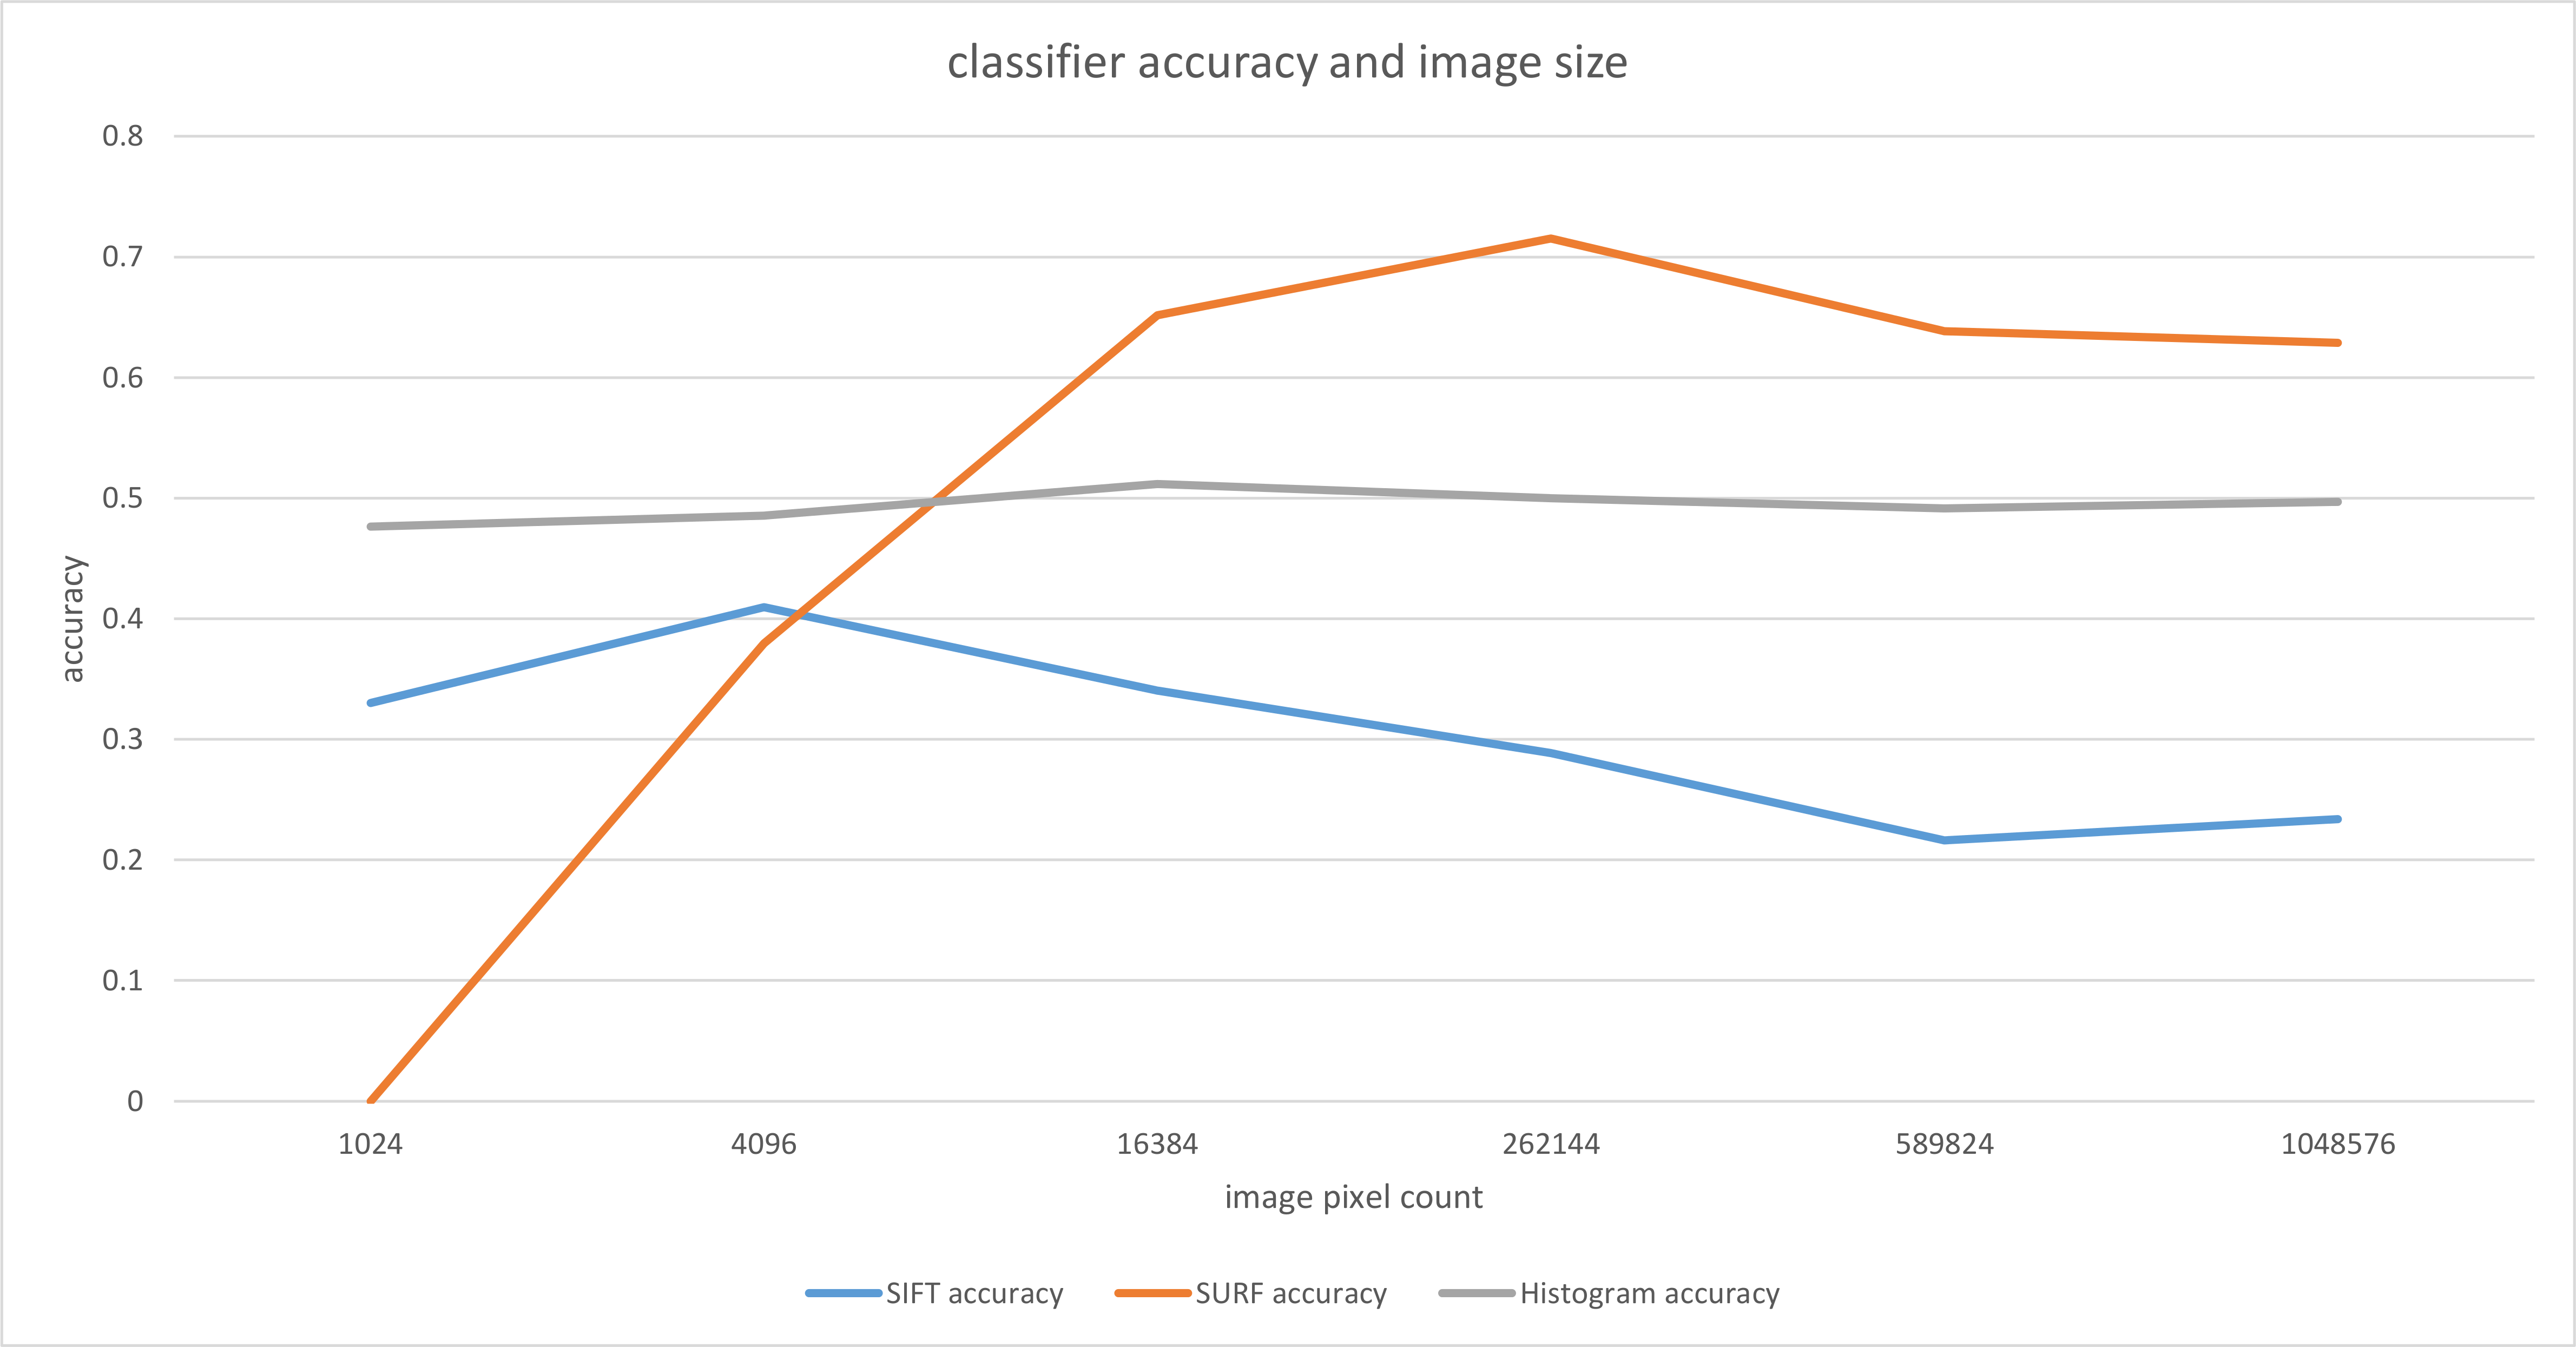
\includegraphics[scale=0.6]{figures/results_resolution}		
		\caption{Impact of image size on histogram, SIFT and SURF classifier performance. Test details: HI-6, SI-6, SU-6}
		\label{fig:resultsResolution}
	\end{figure}
	Different image resolutions were tested on SURF, SIFT and color histograms to determine if a higher image resolution automatically means a higher accuracy. Intuitively, image size or resolution should be a classical tradeoff between computational cost and classification performance. To test if higher resolutions yield better accuracies, 6 resolutions were tested from 1024 pixels {(equals a $32 \times 32$ image)} to 1,048,576 pixels {($1024 \times 1024$)}. The results are visualized in figure \ref{fig:resultsResolution}.  
	
	Up to a certain point the accuracy of SIFT and SURF gets better until it drops and levels out. Since for every test run the number of extracted descriptors for the classification was the same, it is not the quantity of keypoints that affects the performance but the quality. SURF extracts fewer keypoints on small images. For the 1024 image size SURF was not able to detect even one keypoint for most of the images which means that for smaller images the algorithm has to sample more random keypoints which are lower quality keypoints and decrease performance. SIFTs keypoint detector seems to have less problems with smaller images and increasing the image size only slightly increases performance. For big images the accuracy is decreasing again which may be due to fact that the number of extracted keypoints increases but the actual number of used keypoints remains the same so potentially more stable keypoints are filtered out.
	
	Just changing the image size does not impact performance for histograms since the number of image segments does not change so the extracted histogram is always the same regardless of the image size. This is further proven by 40 random tests {(HI-7)} on the histogram parameters: number of histogram bins, image segments and the image size. Figure \ref{fig:resultsResolutionHistogram}a shows that even with different numbers of bins or image segments the image size has no impact on performance at all. However, there is a significant positive correlation {(correlation coefficient: $+0.538$, p-value: $0.00034$)} between the length of the feature vector and the accuracy {(fig. \ref{fig:resultsResolutionHistogram}b)}.
	
	\begin{figure}[htb]
		\centering
		\subfloat[Image size]{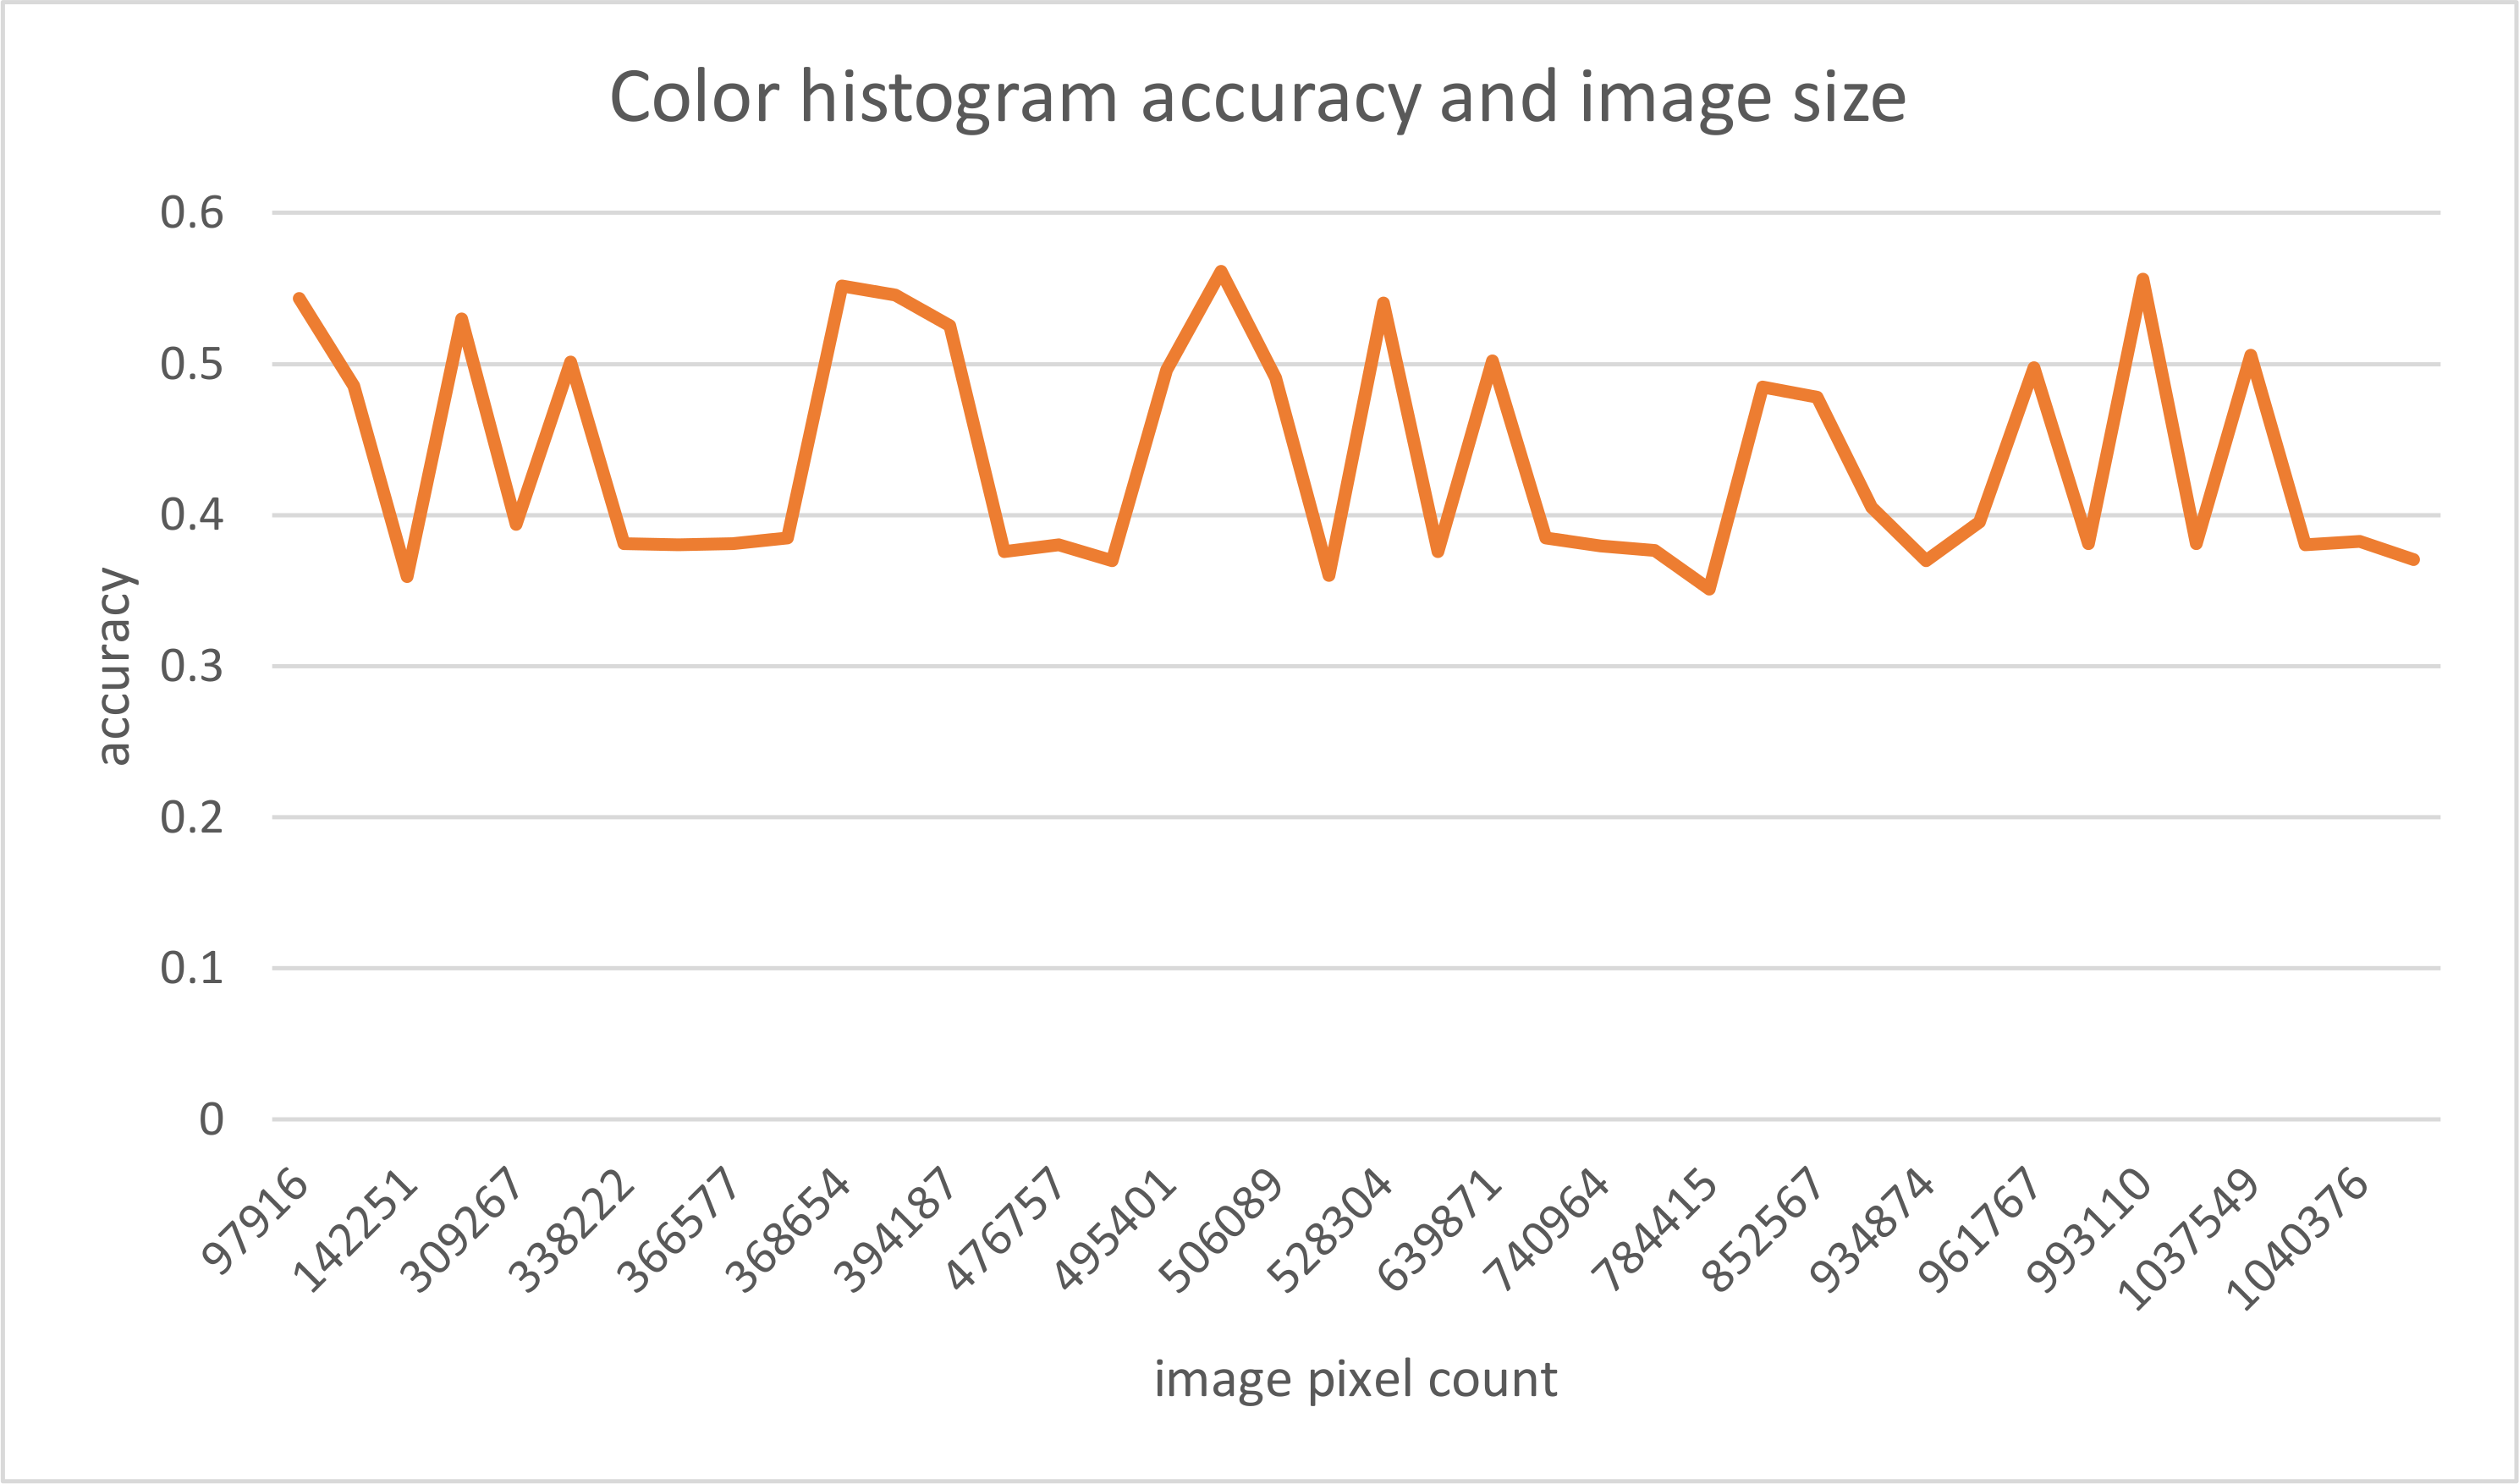
\includegraphics[width=75mm]{figures/results_h7ImageSize}}
		\subfloat[Feature vector length]{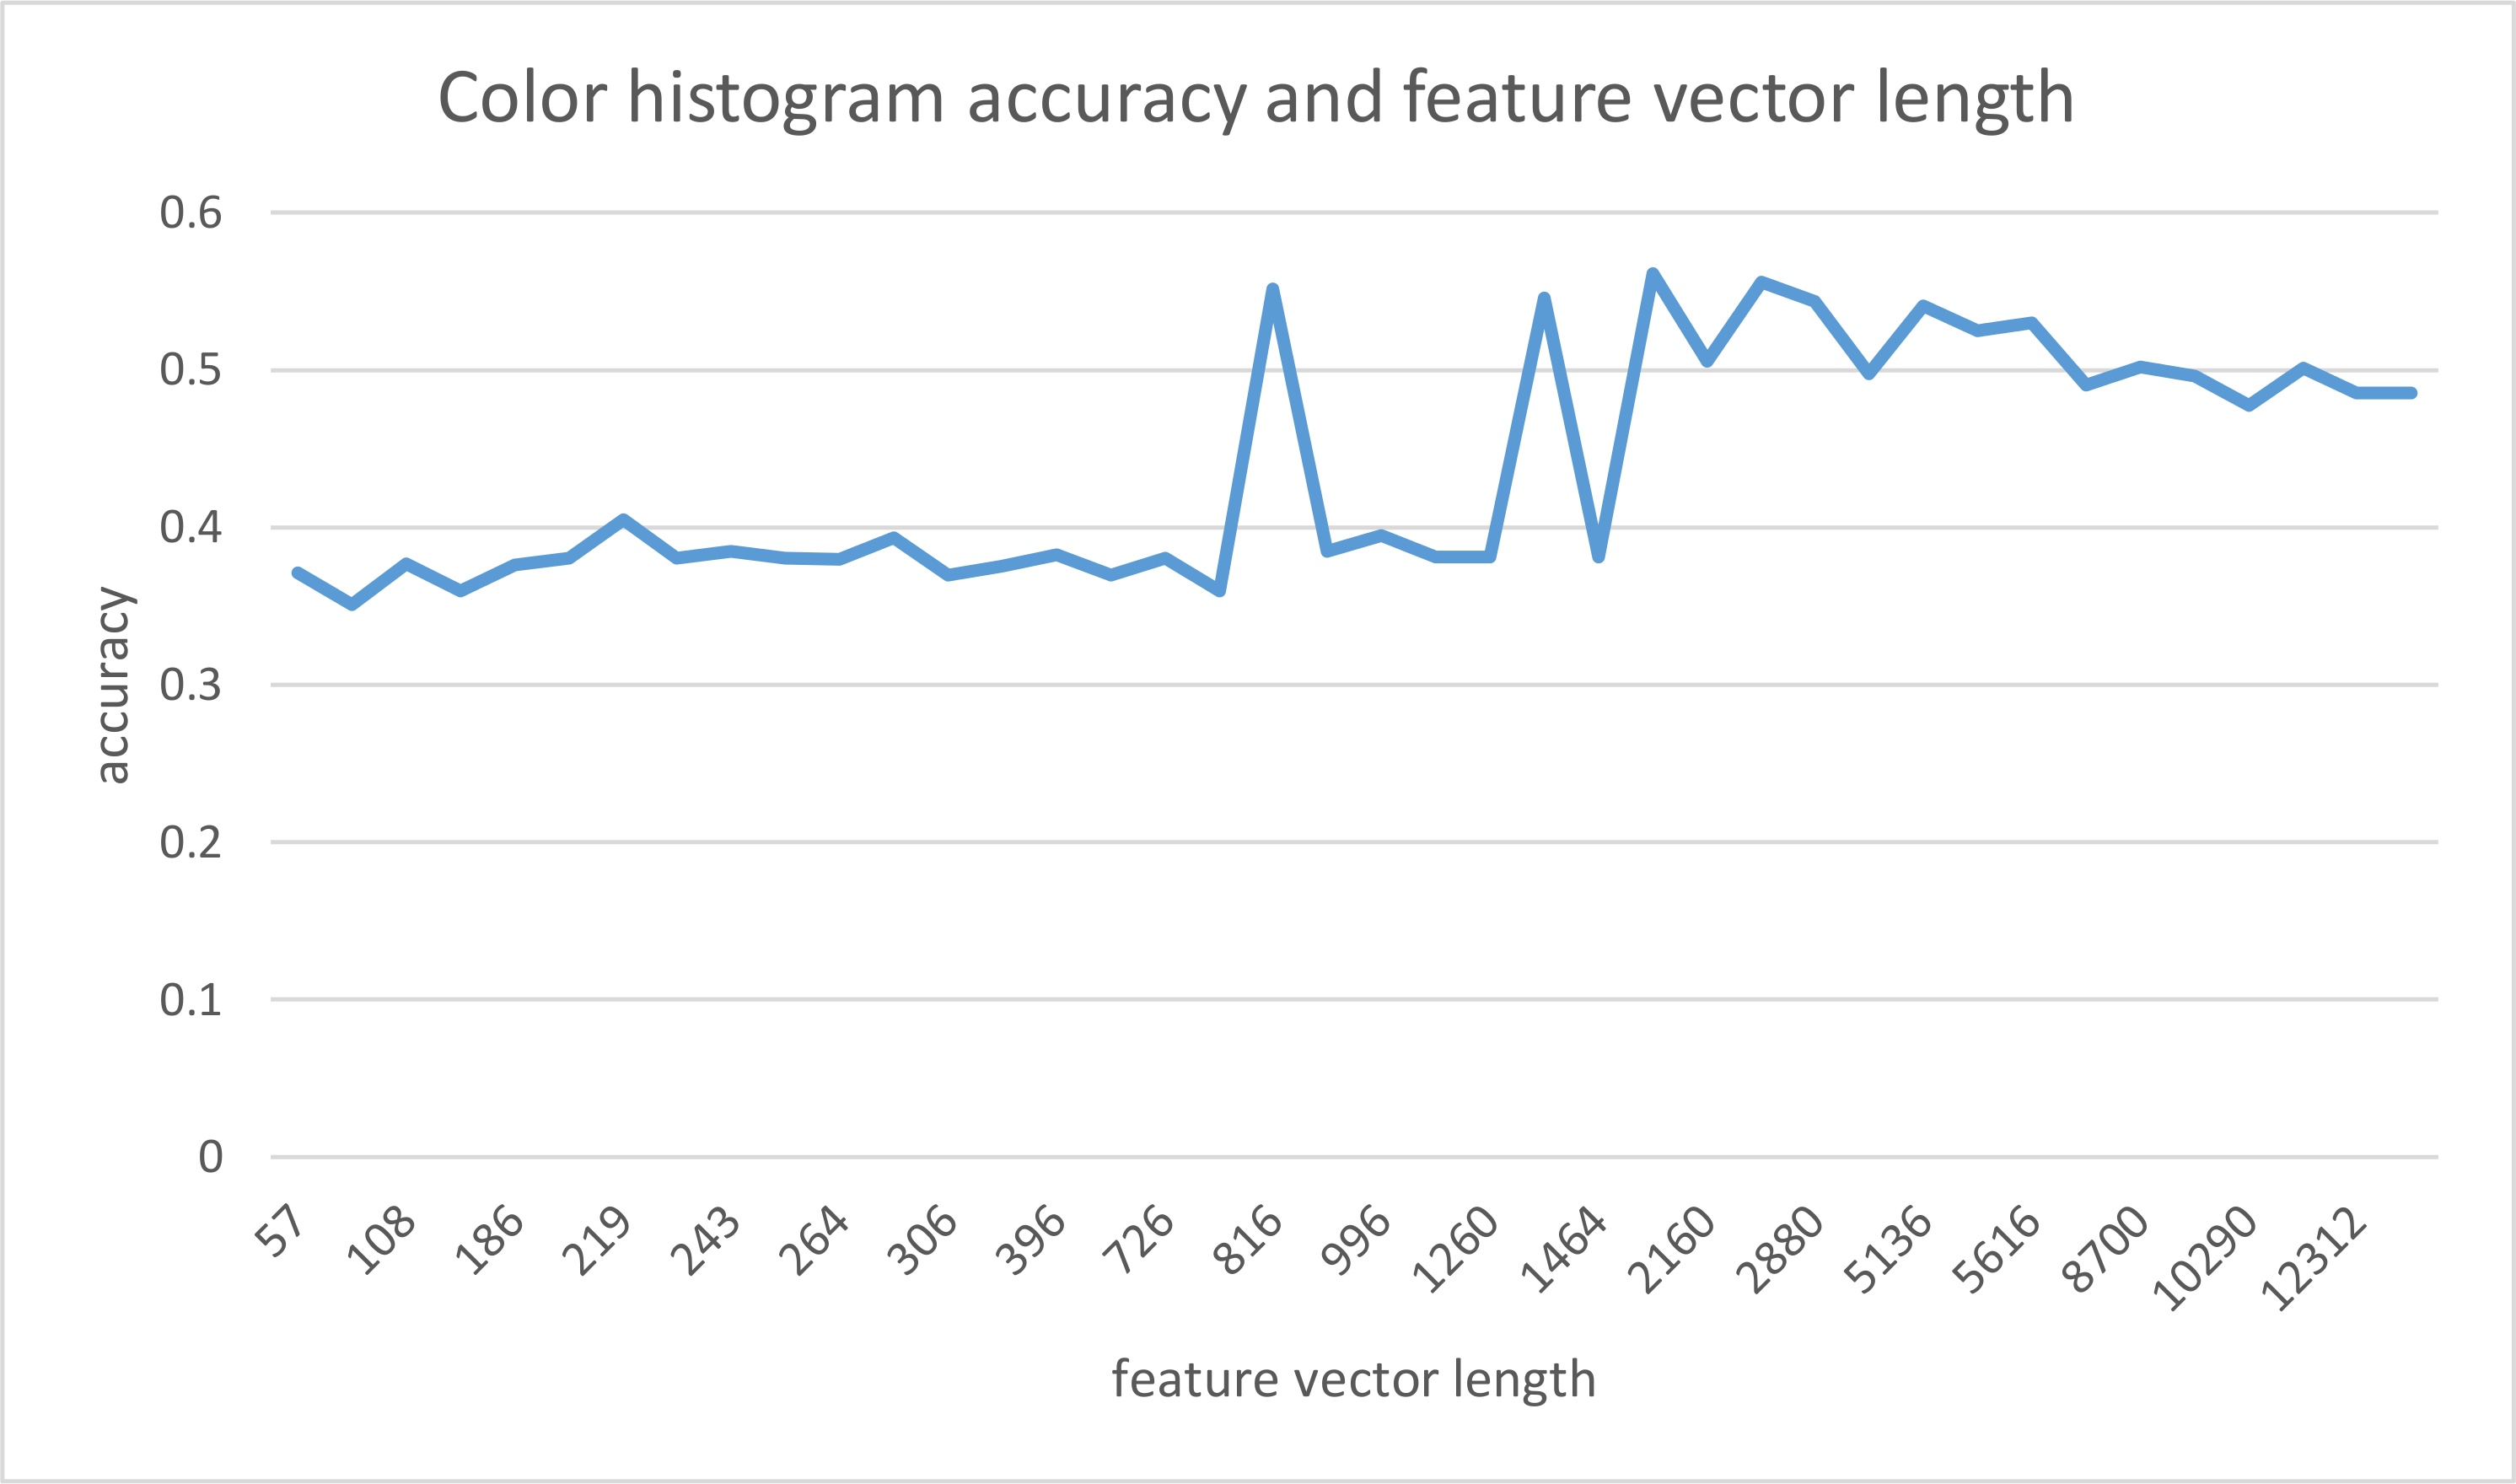
\includegraphics[width=75mm]{figures/results_h7FeatureVector}}
		\caption{Histogram classifier performance under the impact of number of bins, image segments and image size. Test details: H-7}
		\label{fig:resultsResolutionHistogram}
	\end{figure}
			
	\subsection{Number of Extracted Keypoints}
	\begin{figure}[htb]
		\centering
		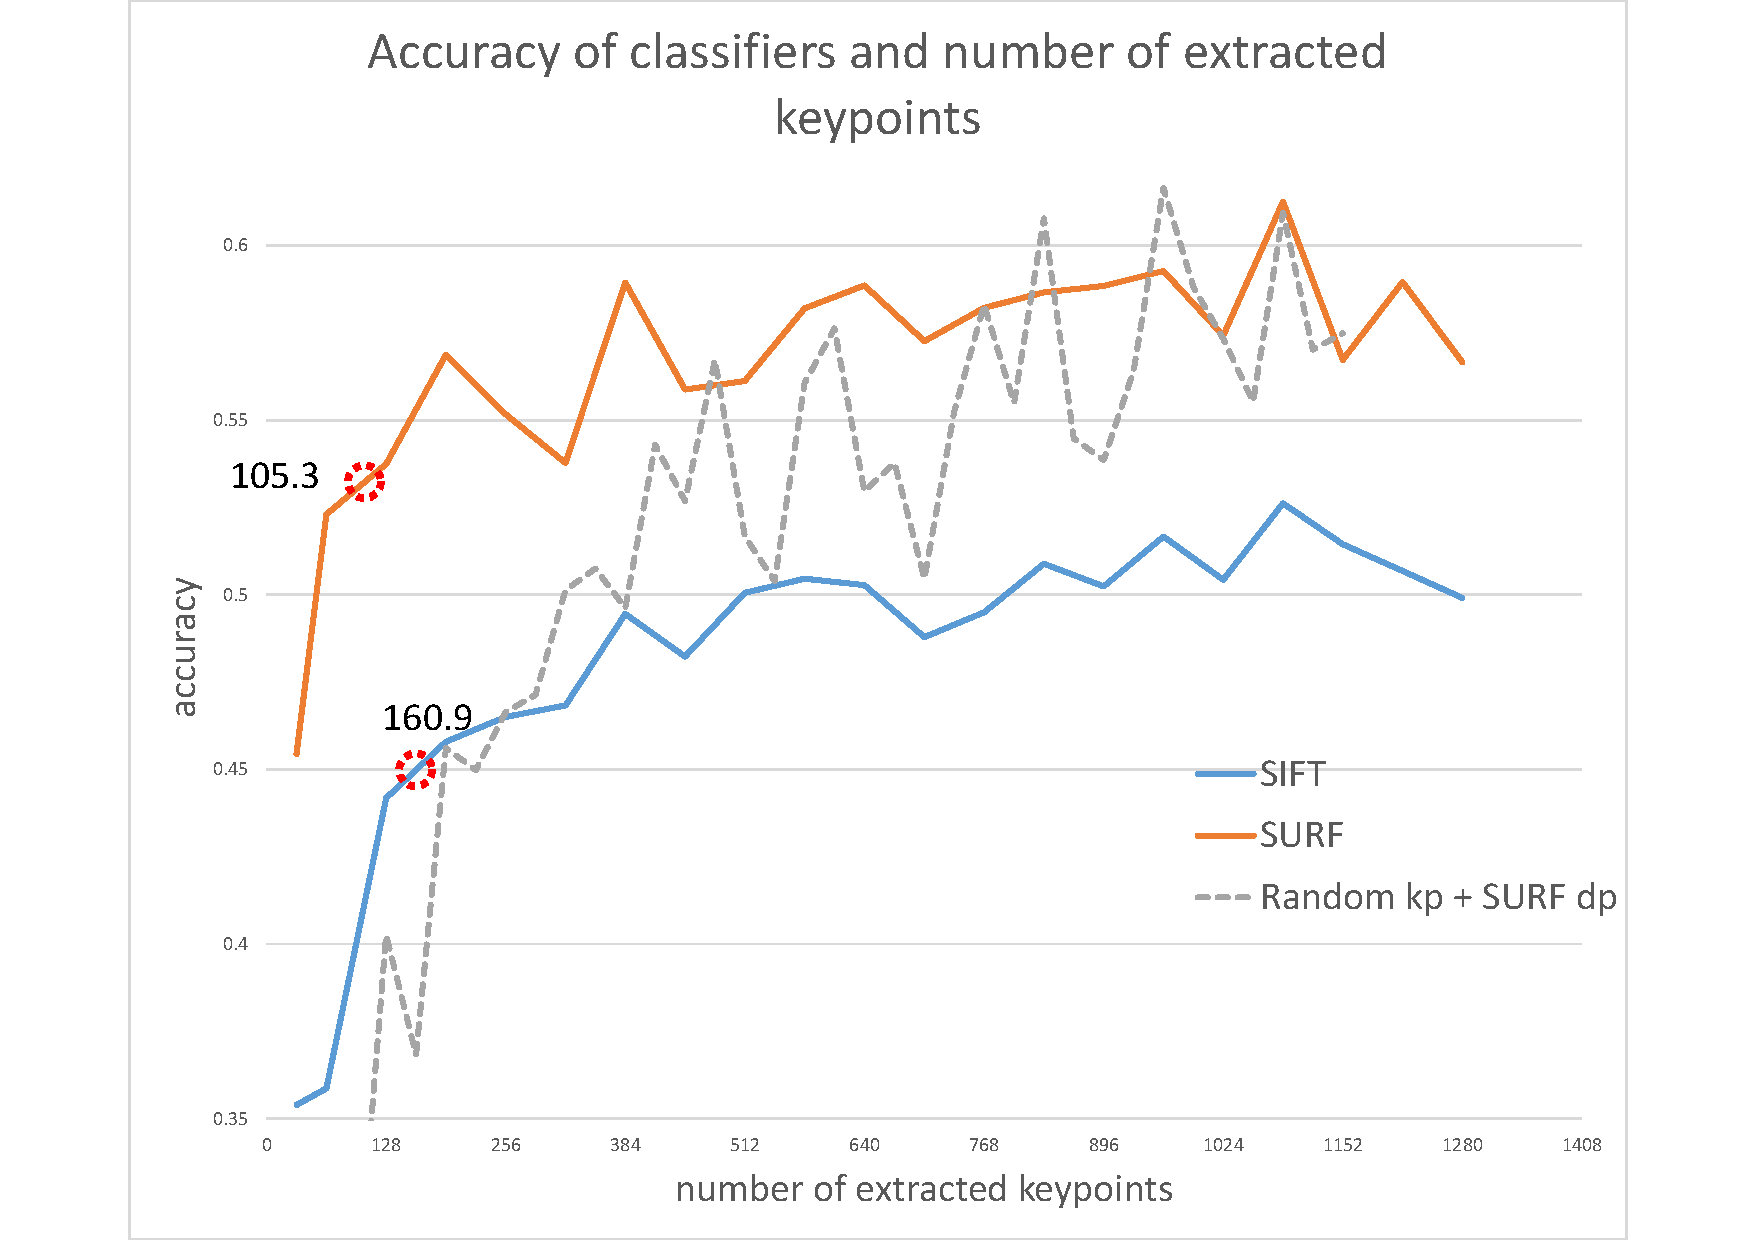
\includegraphics[scale=0.4]{figures/results_keypoints}		
		\caption{Impact of keypoint quantity on SIFT and SURF accuracy. The red circle denotes the number of mean extracted keypoints for this classifier. Test details: SI-1, SU-1, R-1}
		\label{fig:resultsKeypoints}
	\end{figure}
	The number of extracted keypoints is basically the length of the extracted feature vector. Each keypoint produces a 128 dimensional vector in case of SIFT and a 64 dimensional vector for SURF. 
	
	Deciding on a fixed number of keypoints is a very difficult problem because the quality and quantity of extractable keypoints is dependent on many various parameters like contrast and edge thresholds or image size. Figure \ref{fig:resultsKeypoints} shows the change in accuracy for changes in the number of used keypoints. Other parameters are the same over all iterations. There is a positive correlation for both SIFT and SURF between number of keypoints and accuracy which means that up to a certain point adding more keypoints helps to improve performance. 
	
	Intuitively, the performance degrades after a certain point because the keypoint detectors can't extract enough relevant points of the region of interest {(food item)} so more irrelevant points of background objects have to be included. After the background points are all included the missing points have to be randomly augmented which should decrease performance even more.
	
	The tests were performed with an image resolution of 16,384 pixels which corresponds to a size of $128 \times 128$. For this specific image size and the 8-class Food-100 subdataset SURF detects a mean of 105.3 keypoints per image {(red circle)} which means that after 105 keypoints in this test most of the other points were randomly sampled but the accuracy increased nonetheless. For SIFT the mean number of detected keypoints per image is 160.9. So the prior assumption that randomly sampled keypoints decrease performance is not completely correct. Though the gradient of the performance increment is much less after this point than the increment with real sampled keypoints before.
	
	To compare the two keypoint extractors and further proof this assumption, a third and fourth test were performed. In these tests all keypoints were randomly sampled around the image center so no edge detection was performed. For keypoint description SURF was used in the third test and SIFT was used in the fourth test {(not shown in figure \ref{fig:resultsKeypoints})}. The gray dotted line in figure \ref{fig:resultsKeypoints} shows the random test with the SURF feature descriptor. These tests make it possible to derive the following assumptions:
	
	\begin{enumerate}
		\item Detected keypoints allow for a higher accuracy than randomly sampled keypoints because it takes a long time for the random keypoint sampler to catch up with the performance of the SURF or SIFT classifier.
		\item The random sampler does not use an edge detector. Only the SURF/SIFT descriptors are used. This makes it possible to compare the performance of the descriptors since it takes the detectors out of the equation. For this specific task it seems that SURF is not only the faster descriptor but also more accurate in describing an image.
		\item Random keypoint sampling is a positive alternative for images with low contrast values were detectors are not able to sample many keypoints.
	\end{enumerate} 
	
		
	\subsection{Keypoint Filtering}
		\begin{table}[htb]
			\centering
			\begin{tabular}{@{}ccc@{}}
				\toprule
							 & SIFT  & SURF  \\ \midrule
				Filtering    & 0.568 & 0.568 \\
				No filtering & 0.440 & 0.599 \\ \bottomrule
			\end{tabular}
			\caption{Results of keypoint filtering for SURF and SIFT. Test details: SU-3, SI-3}
			\label{tab:resultFiltering}
		\end{table}
	
	The algorithm proposed in section \ref{subsub:keypointFiltering} filters keypoints by weighting their response values with the distance to the image center. As table \ref{tab:resultFiltering} shows, this dramatically improves the performance of SIFT from 0.44 to 0.57. For SURF, however, the filtering does even reduce the accuracy although filtering SURF keypoints should also be applicable since the SURF keypoint detector produces even more false positive keypoints than SIFT which is shown in figure \ref{fig:ResultsKeypointFiltering}. So while this feature may not useful for SURF keypoints it is still effective for SIFT.  
	
	\begin{figure}[htb]
		\centering
		\hspace{\fill}%
		\subfloat[1102 unfiltered \gls{surf} keypoints]{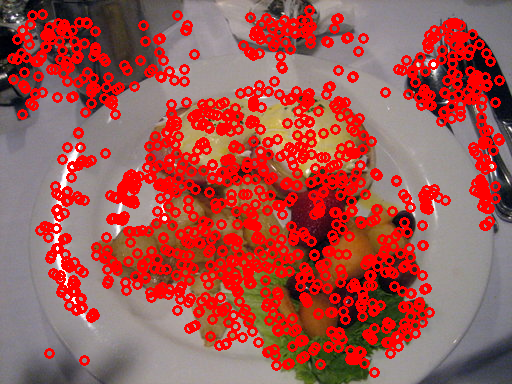
\includegraphics[width=35mm]{data/images/results/resultsSURF_noFiltering}}
		\hspace{\fill}%
		\subfloat[500 filtered \gls{surf} keypoints]{\includegraphics[width=35mm]{data/images/results/resultsSURF_filtering}}
		\hspace{\fill}%
		\subfloat[835 unfiltered SIFT keypoints]{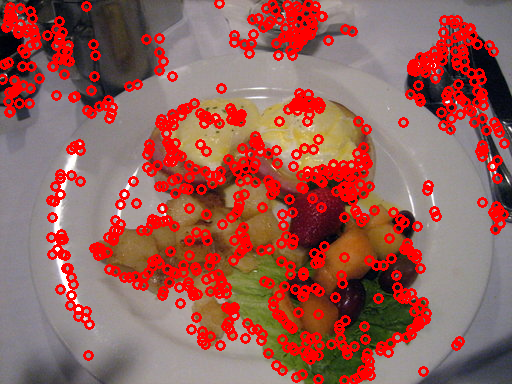
\includegraphics[width=35mm]{data/images/results/resultsSIFT_noFiltering}}
		\hspace{\fill}%
		\subfloat[500 filtered SIFT keypoints]{\includegraphics[width=35mm]{data/images/results/resultsSIFT_filtering}}
		\hspace{\fill}%
		\caption{Comparison of \gls{sift} and \gls{surf} keypoint filtering.}
		\label{fig:ResultsKeypointFiltering}
	\end{figure}
	
	\subsection{Bag of Words Dimension}
	\begin{figure}[htb]
		\centering
		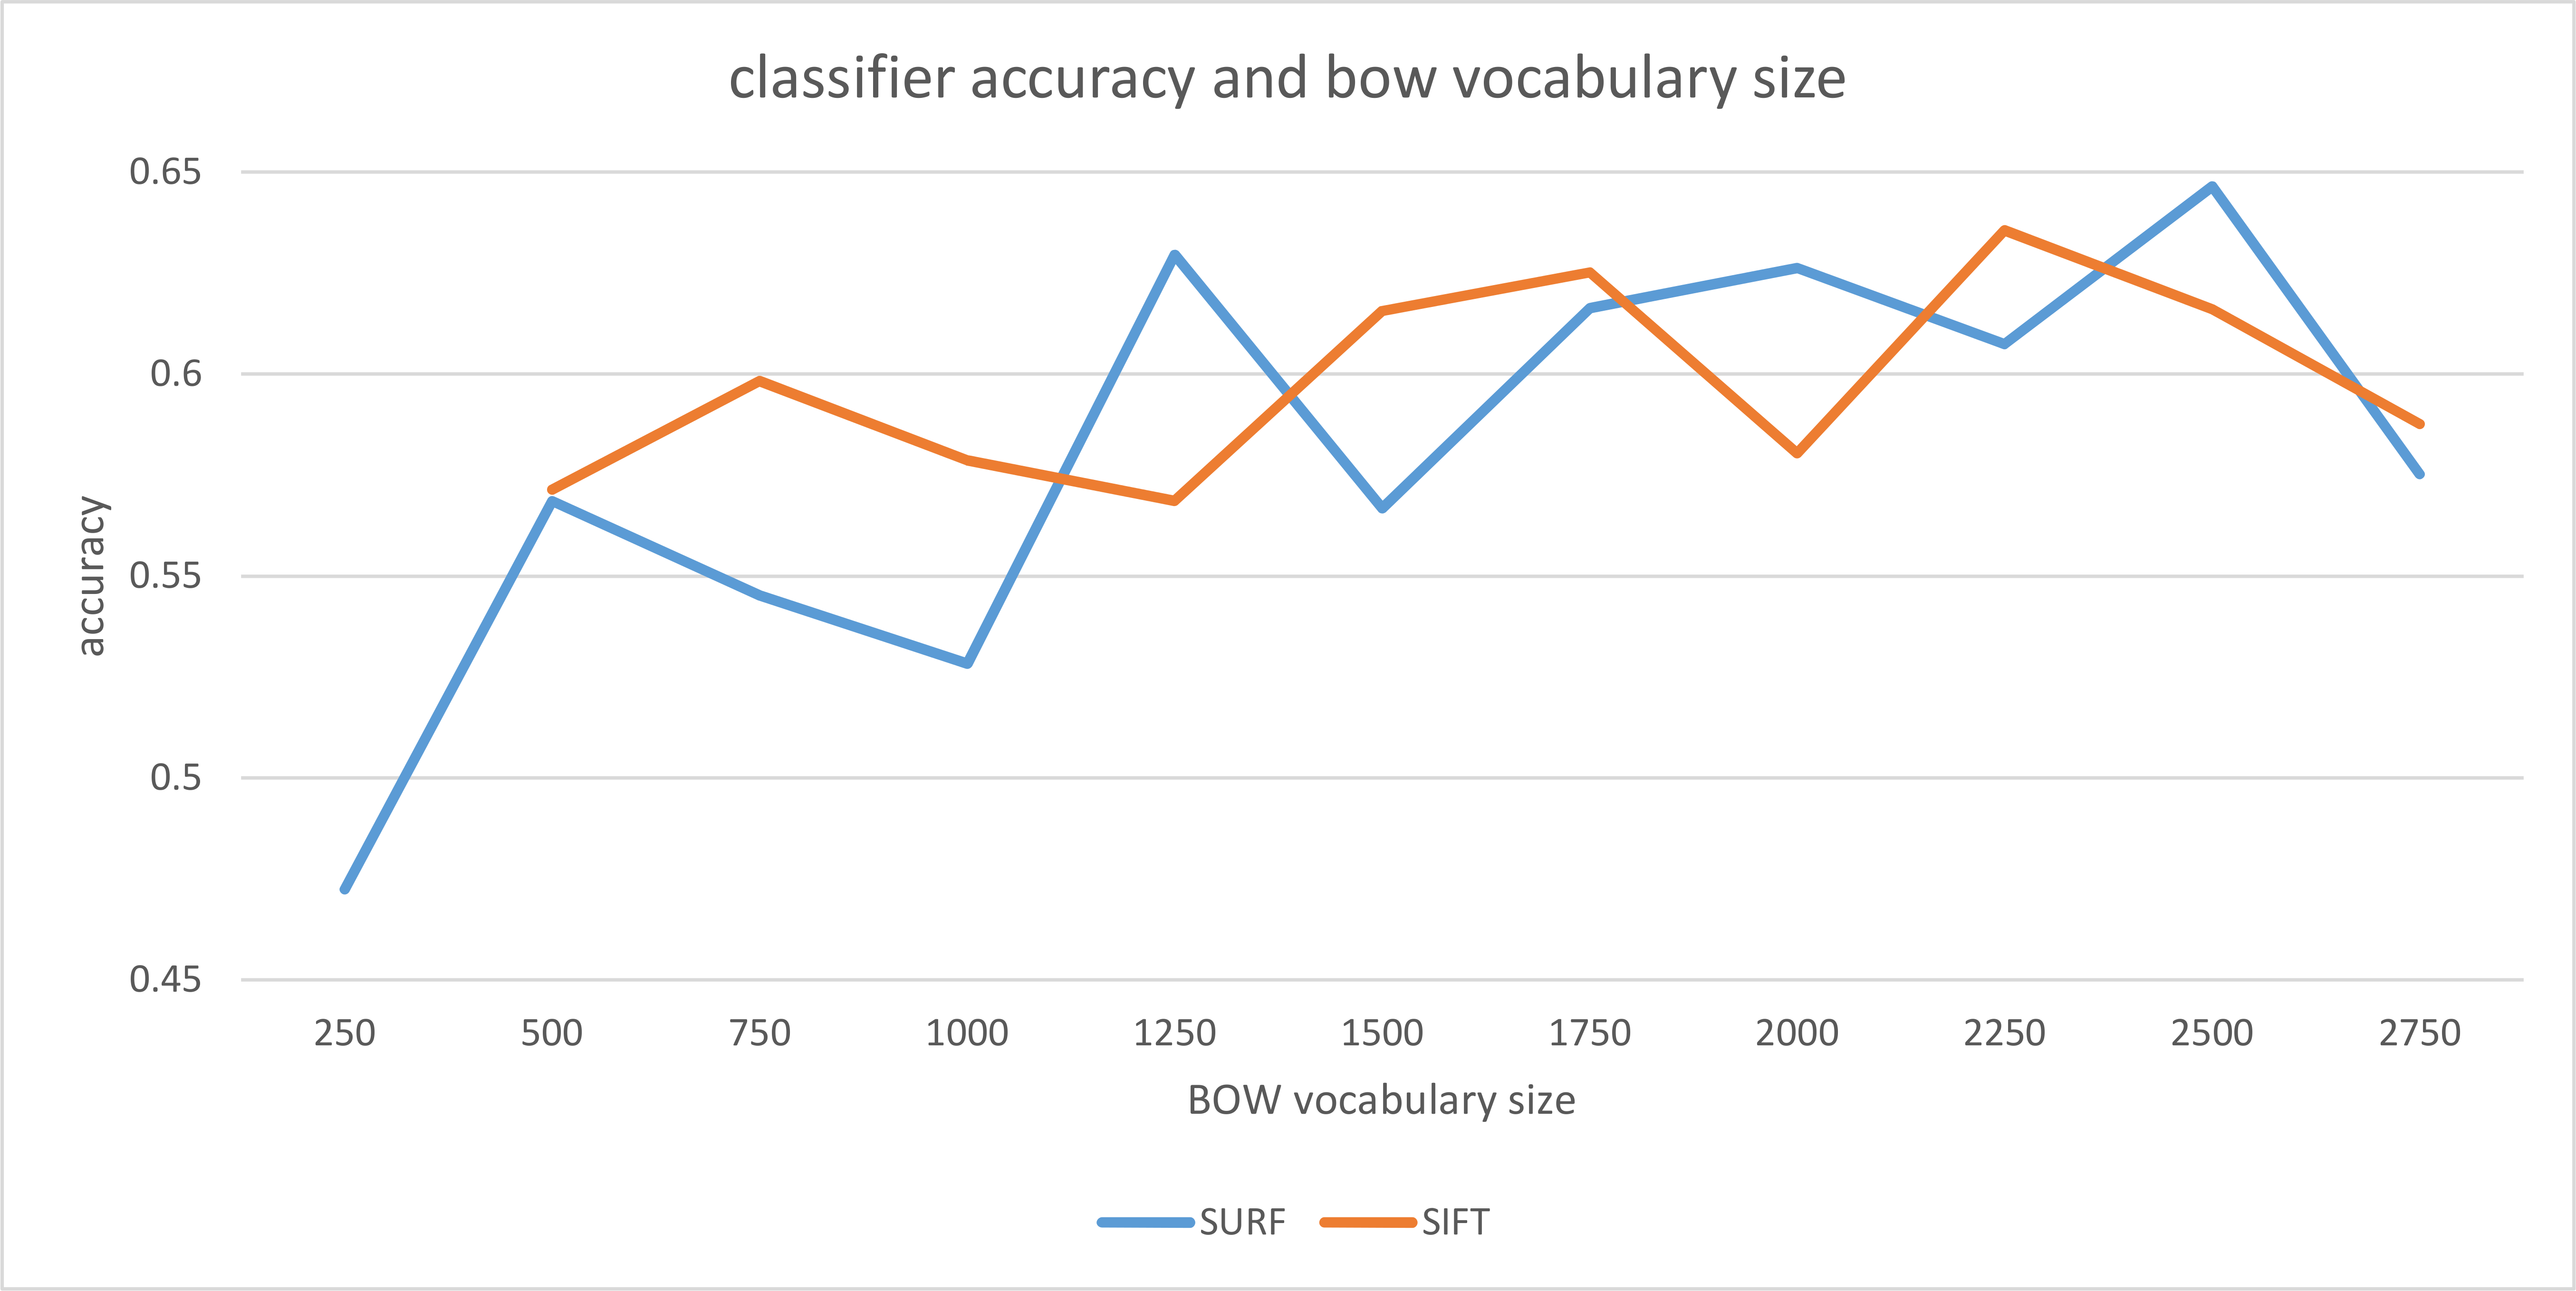
\includegraphics[width=\linewidth]{figures/results_bow}		
		\caption{Impact of bow vocabulary size on SIFT and SURF classifier performance. Test details: SI-2, SU-2}
		\label{fig:resultsBow}
	\end{figure}
	The size of the bag of words vocabulary is a very important parameter because the \gls{bow} histogram is the actual feature vector that is used for classification and not the feature vector from classifiers like SIFT or SURF. A bad \gls{bow} vocabulary can lead to poor classification performance even if the input feature vectors are good. One way to influence the \gls{bow} vocabulary is its size. Figure \ref{fig:resultsBow} visualizes the impact of the vocabulary size on the overall performance of the classifier. The best accuracy was achieved with a vocabulary size of 2250 for SIFT and 2500 for SURF. For SURF there is a significant positive correlation {(correlation: 0.695, p-value: 0.018)} between the vocabulary size and the accuracy in the interval $[250, 2750]$. The correlation of SIFT is not significant enough {(p-value: 0.063)}. Although the classifier performance for bigger vocabularies is higher, it is not feasible to use huge vocabularies since the training time also increases with an increasing \gls{bow} size.
	
	\subsection{Neural Networks}
			
	Training and performance of neural networks hugely depends on the selected architecture. In the course of this thesis 9 models were evaluated on small datasets. On the one hand, small datasets allow for fast training but on the other hand, neural networks need as many samples as possible and the dataset the neural nets were tested on were 8 classes from the 50-data dataset which only contains 100 images per class. The result of a relatively small convolutional neural network is shown in figure \ref{fig:overfittingNet}a and could serve as a perfect example of overfitting. The training and validation error both decrease till epoch 80. After the 80th epoch the training error continues to decrease but the validation error stagnates and even begins to increase after the 250th epoch.
	
	\subsubsection*{Dropout}
	\begin{figure}[htb]
		\centering
		\subfloat[No dropout]{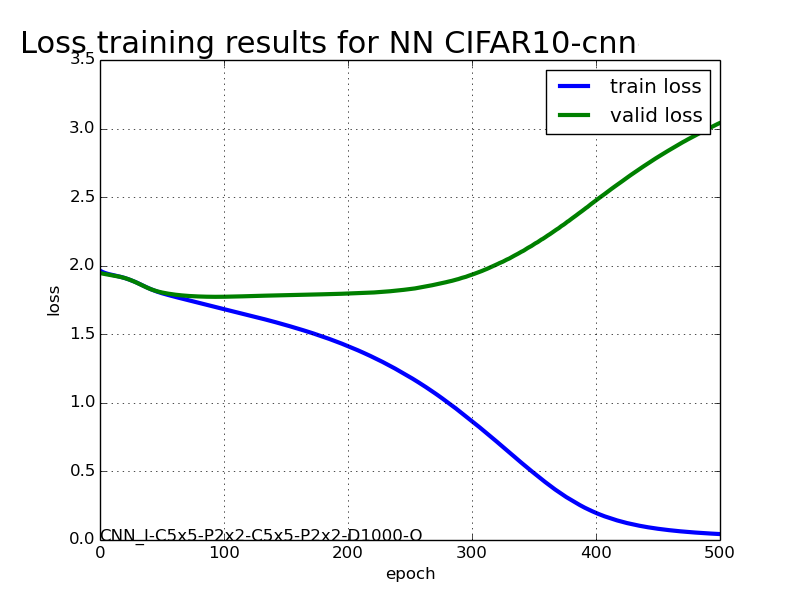
\includegraphics[width=75mm]{figures/resultsCIFAR10_trainingLoss}}
		\subfloat[Two different dropout values]{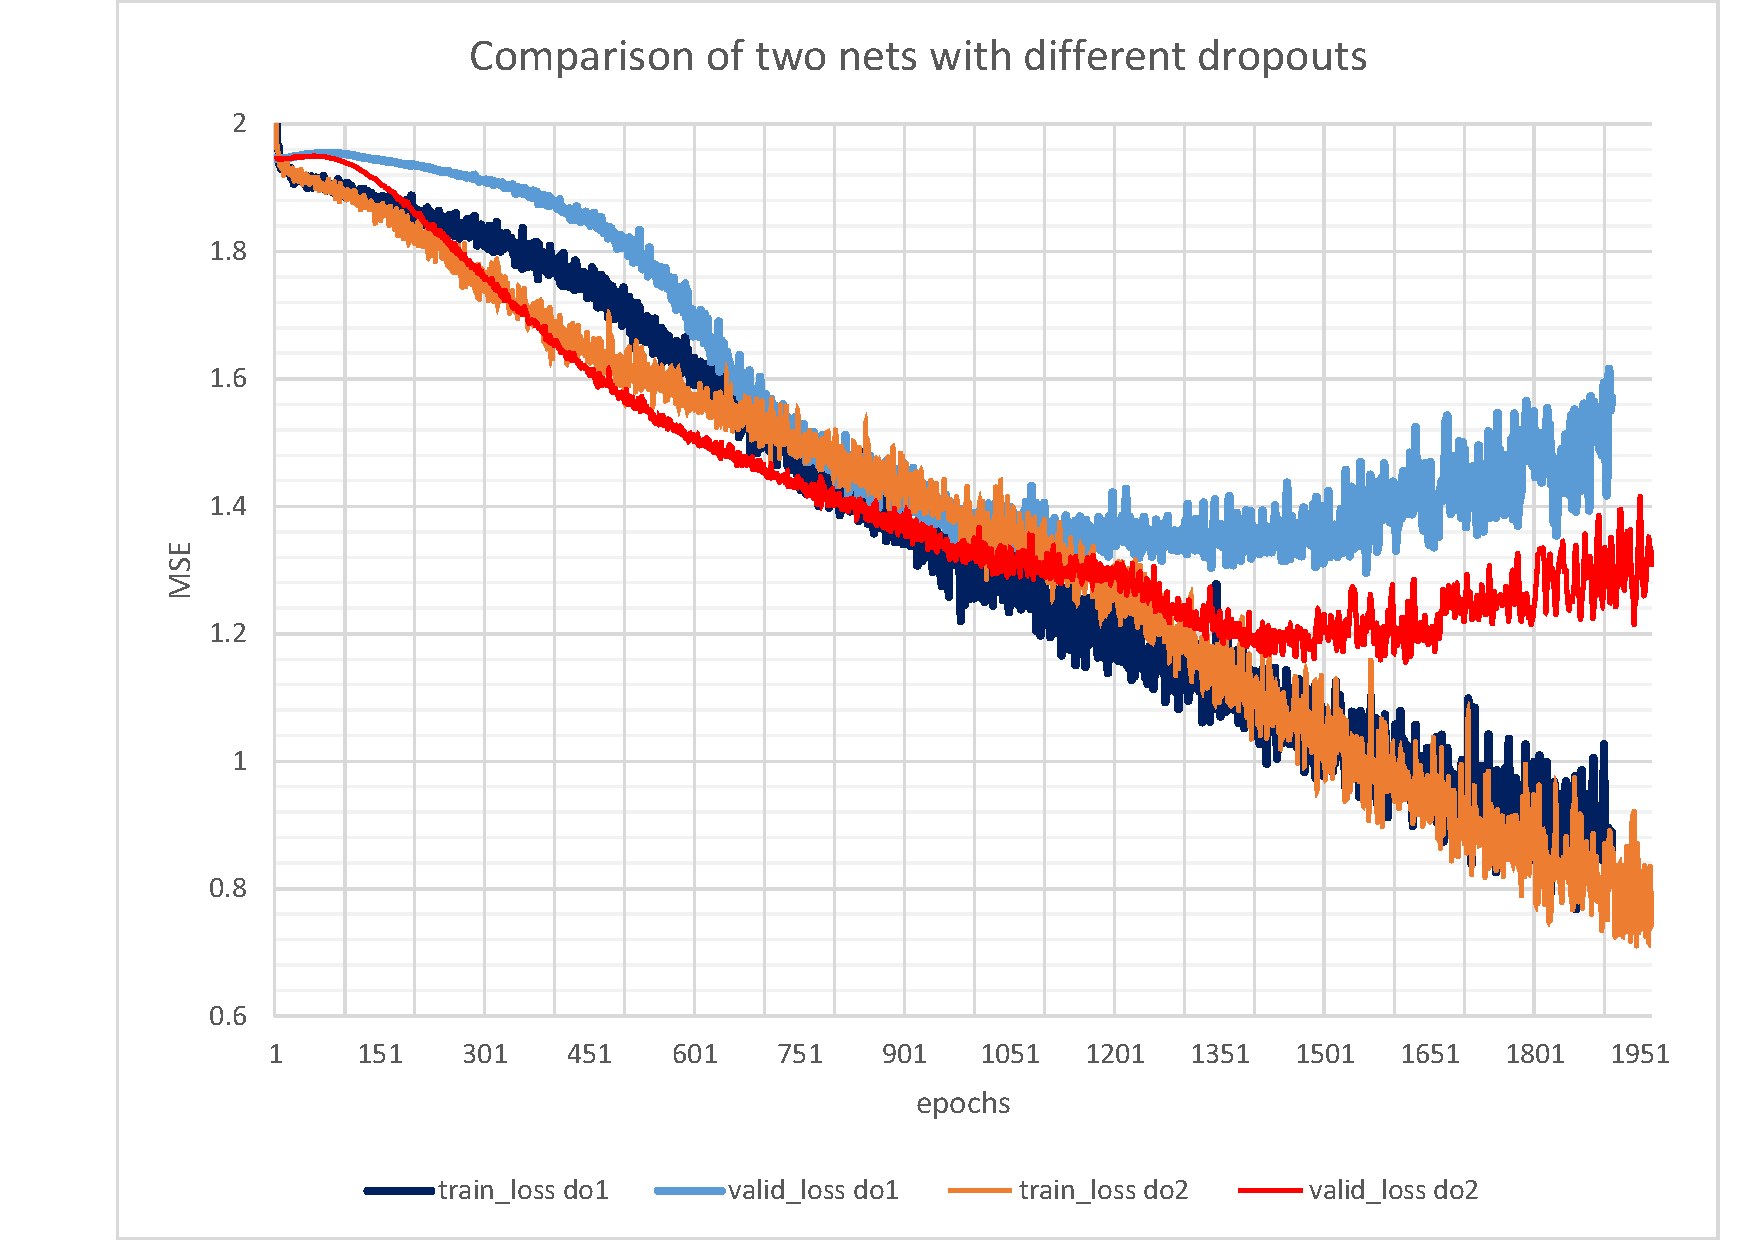
\includegraphics[width=75mm]{figures/resultsCIFAR10_dropout}}
		\caption{Three different dropout settings on a small net which was originally used for training on CIFAR-10.}
		\label{fig:overfittingNet}
	\end{figure}
	A way to reduce overfitting is dropout {(see section \ref{subsec:overfittingDropout})}. Figure~\ref{fig:overfittingNet}b shows the training loss of two networks with same architecture as in figure \ref{fig:overfittingNet}b only this time with dropout applied before and after the dense layers. The blue lines correspond to a network with 0.5 dropout applied and the red and orange lines represent a network with 0.6 dropout applied. This time the network overfits much later than before and until epoch 1000 the validation loss for the second dropout setting is even less than the training loss. This is due to the fact that the dropout is only applied on the training data and not on the validation data.

	
	\subsubsection*{Data Augmentation}
	
	To further reduce overfitting and improve performance, augmentation on the data is performed {(see section \ref{subsec:dataAugmentation})}. Similar to the network with dropout in figure \ref{fig:overfittingNet}b, the validation loss is significantly lower than the testing loss. This is caused, because data augmentation is only applied on the training data. Depending on the \gls{cpu} and \gls{gpu} the additional time per epoch for data augmentation may vary but on the Azure virtual machine {(see section \ref{sec:hardware})} the average duration for each epoch increased from 5.41 to 24.1 seconds. Image value modifying operations like brightness or saturation adjustments are very time consuming. Disabling these operations can decrease the duration for each epoch from 24.1 back to 9.3 seconds and since this does not decrease the performance by that much {(in this specific example the loss even decreased. This could be caused by a better weight initialization.)}, the tradeoff between performance and epoch duration is acceptable.
	
	The training error for the network with no augmentation might not be that much higher but even after 1000 iterations the accuracy did not get better than the null score which indicates that the network did not learn at all and only predicted the majority class.
	
	\begin{table}[htbp]
		\centering
		\caption{Impact of data augmentation on the training of a small neural net on a 8-class dataset. All values are taken after 240 epochs of training.}
		\label{tab:result_augmentation}
		\begin{tabular}{lccc}
			\hline
			\multicolumn{1}{c}{} 				& train loss {(\gls{ace})}  & valid loss {(\gls{ace})}  & duration {(seconds)} \\ \hline
			Augmentation    				& 2.069	 	& 2.066		& 24.116 			\\ 
			Augmentation, no value changes  & 2.022		& 2.015     & 9.262
			    			\\ 
			No Augmentation                		& 2.295	& 2.295 	& 5.412		        \\ \bottomrule
		\end{tabular}
	\end{table}

\section{Results for Food Classification}
\begin{figure}[htbp]
	\centering
	\begin{tabular}{cc}
		\subfloat[SIFT]{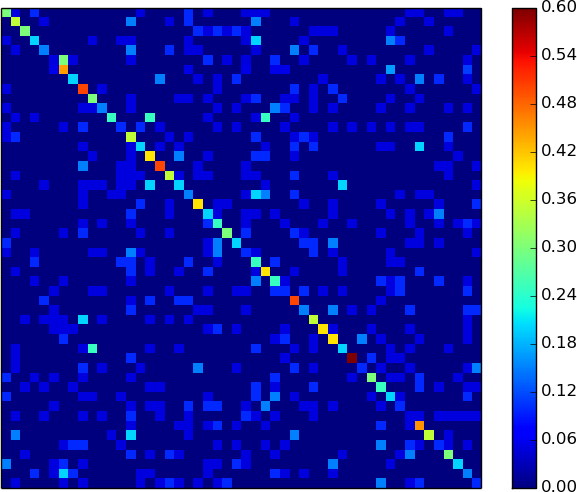
\includegraphics[width=50mm]{figures/results_SIFT_confMatrix}} &
		\subfloat[SURF]{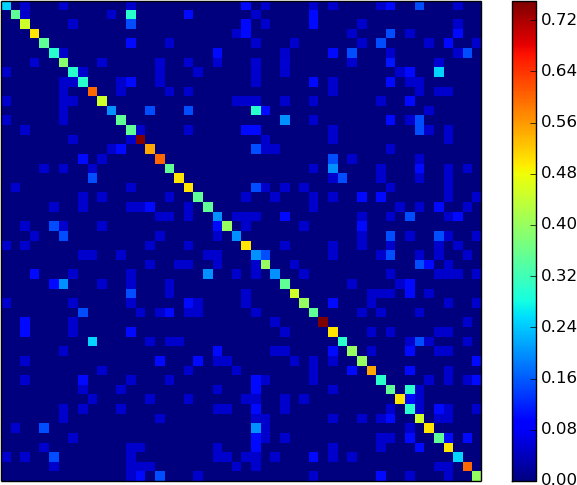
\includegraphics[width=50mm]{figures/results_SURF_confMatrix}} \\
		
		\subfloat[ORB]{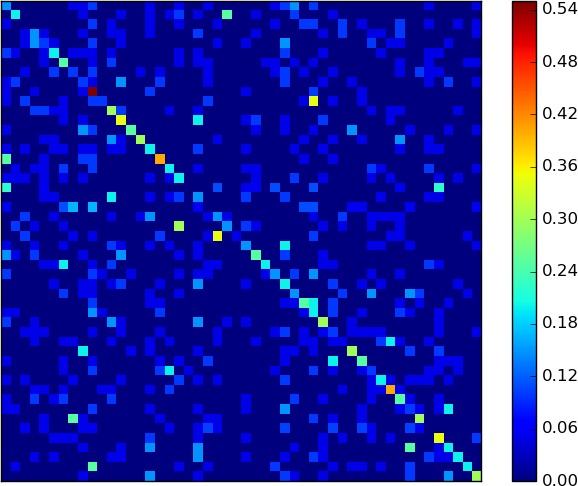
\includegraphics[width=50mm]{figures/results_ORB_confMatrix}} &
		\subfloat[LBP]{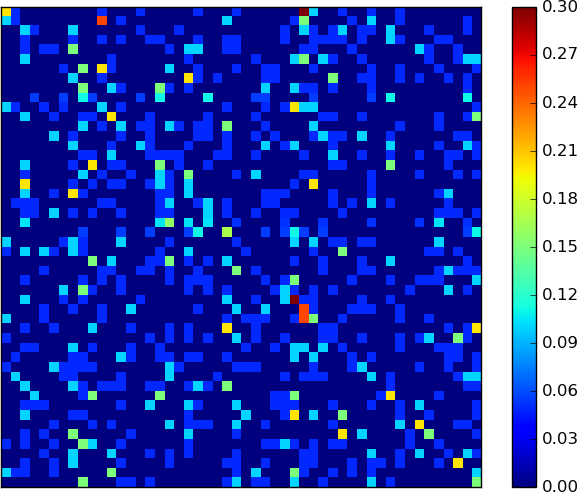
\includegraphics[width=50mm]{figures/results_LBP_confMatrix}} \\
		
		\subfloat[Color Histograms]{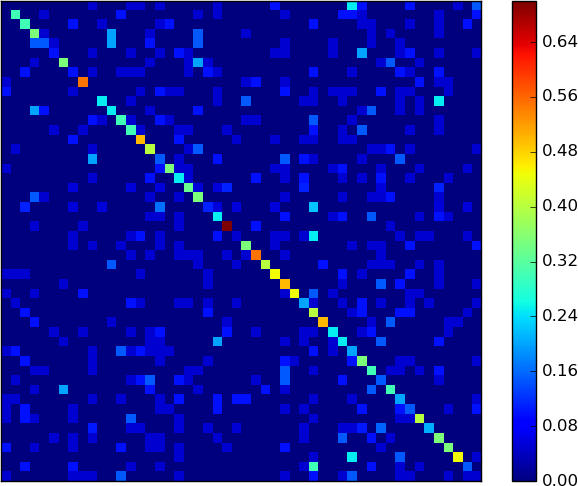
\includegraphics[width=50mm]{figures/results_HIST_confMatrix}} &
		\\
	\end{tabular}
	\caption{Confusion matrix for Top-1 performance on the 50-data dataset validation segment.}
	\label{fig:results_conv}
\end{figure}
In this section the classifiers {(except neural nets)} are tested on the 50-data dataset and table \ref{tab:results} shows the results of this evaluation.

\begin{table}[htbp]
	\centering
	\caption{Evaluation results for feature classifier training on the 50-data dataset.}
	\label{tab:results}
	\begin{tabular}{lccc}
		\hline
		\multicolumn{1}{c}{} 					& Top-1 accuracy  & Top-5 accuracy 	\\ \hline
		\gls{sift} + \gls{bow} + $\chi^2$ \gls{svm}	& 0.3576	 		  & 0.7203			\\ 
		\gls{surf} + \gls{bow} + $\chi^2$ \gls{svm}	& \underline{0.4028}	 		  & \underline{0.7496}			\\ 
		\gls{orb} +  \gls{bow} + $\chi^2$ \gls{svm}	& 0.2011	 		  & 0.5136			\\
		\gls{censure} + \gls{bow} + $\chi^2$ \gls{svm}	& 0.2217	 	  & 0.7341			\\ 
		\gls{lbp} + Poly \gls{svm}					& 0.119	 		  & 0.3036			\\ 
		Color histograms + $\chi^2$ \gls{svm}		& 0.2931		  & 0.6715			\\ \hline
	\end{tabular}
\end{table}


\subsection{SIFT}
\begin{figure}[htbp]
	\centering
	\subfloat[SIFT]{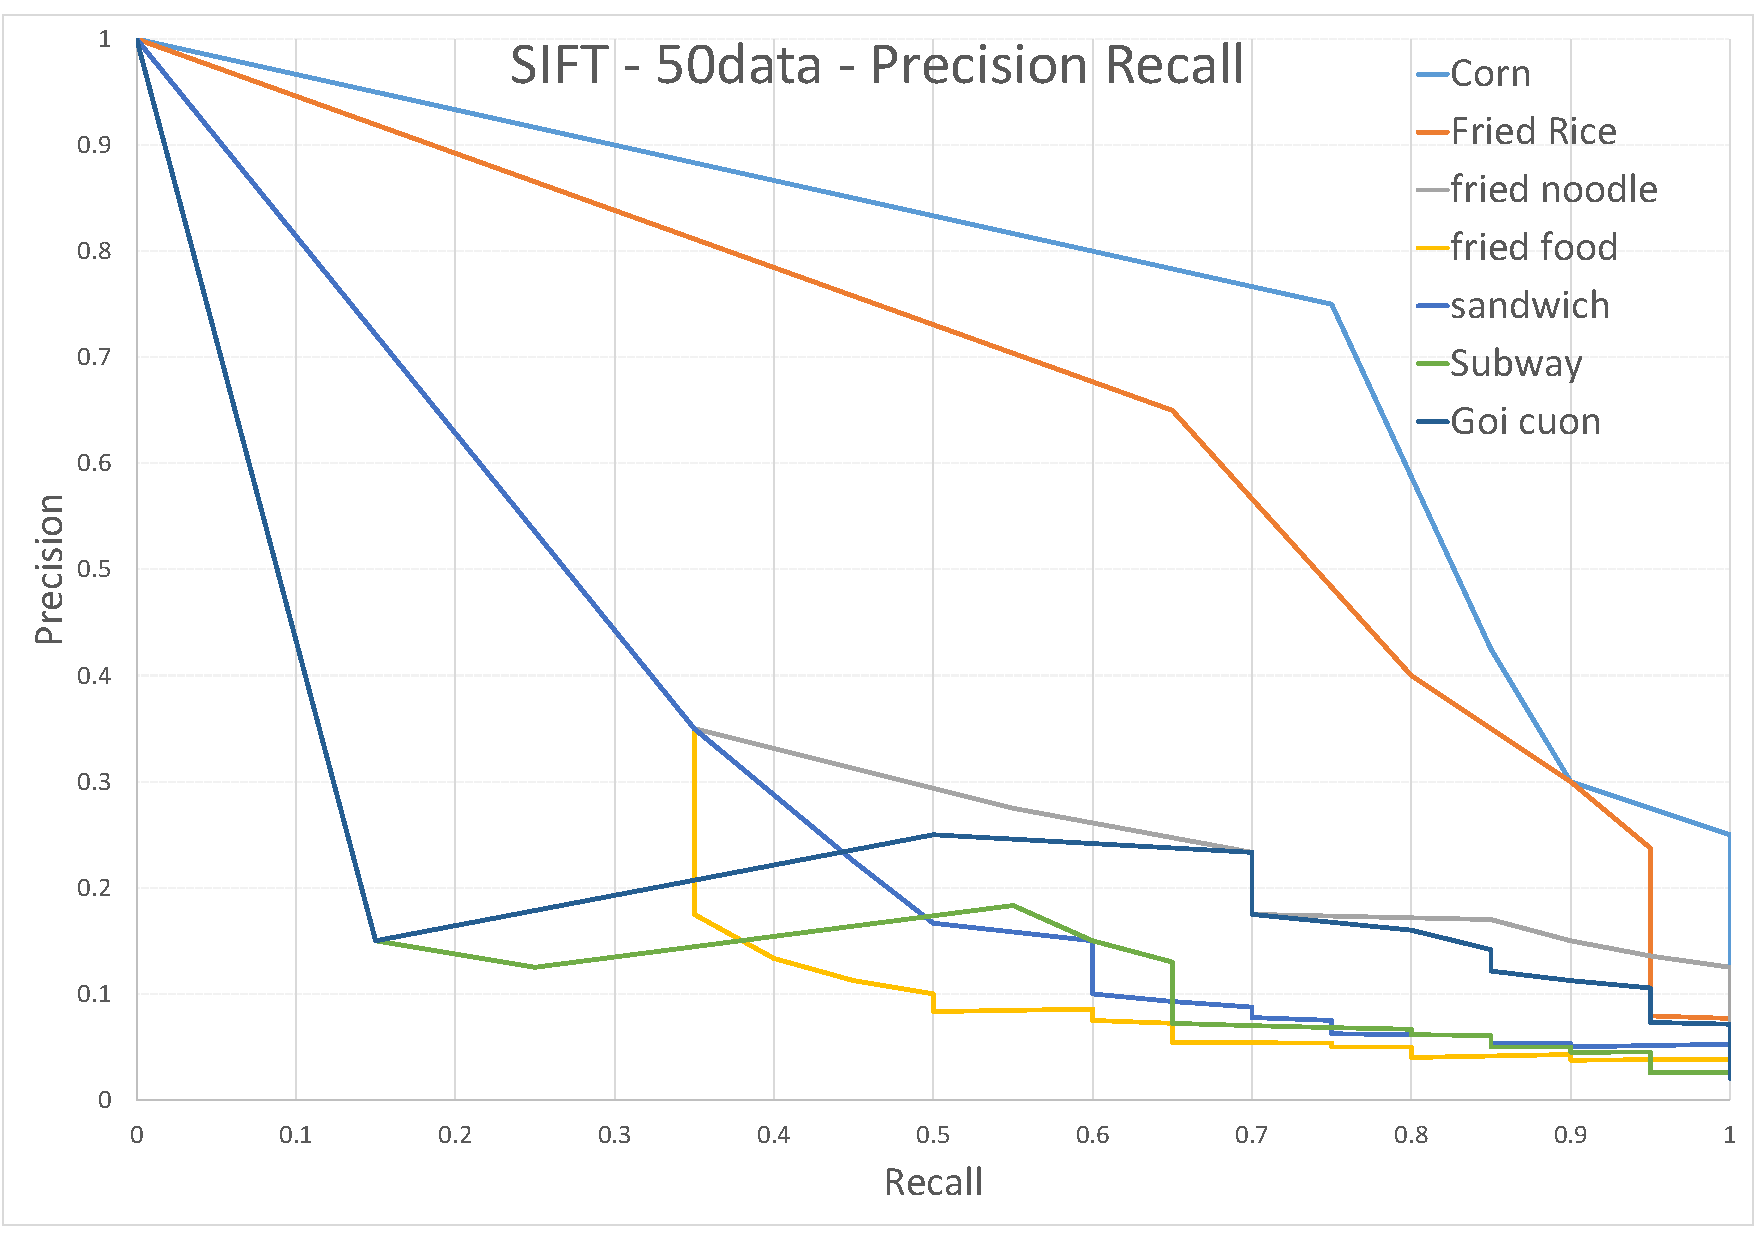
\includegraphics[width=75mm]{figures/results_SIFT_50data_roc}}
	\subfloat[SURF]{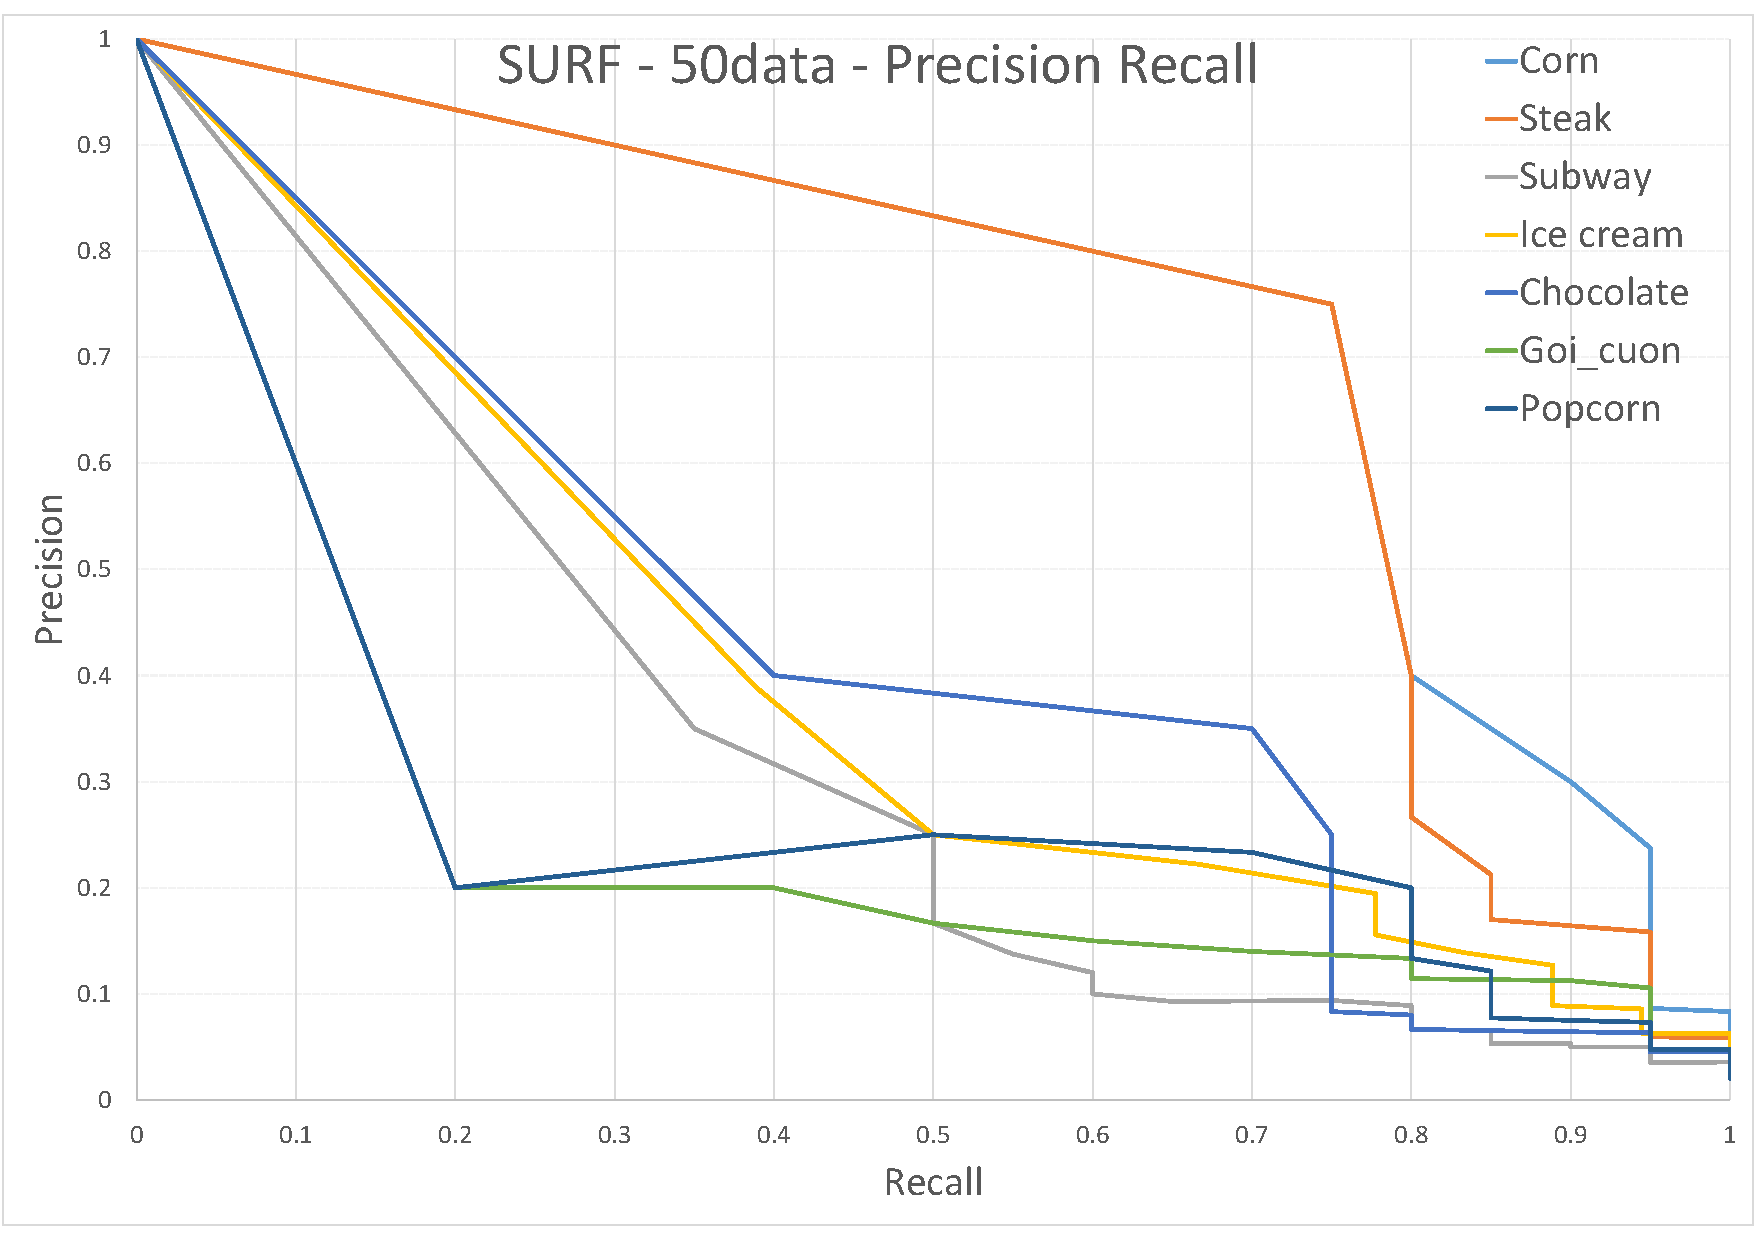
\includegraphics[width=75mm]{figures/results_SURF_50data_roc}}
	\caption{Precision recall curve for SIFT and SURF on the 50data dataset validation segment.}
	\label{fig:results_SIFTSURFroc}
\end{figure}

The \gls{sift} feature classifier was evaluated with an image area size of 262,144 pixels. 1088 weighted and augmented keypoints were extracted. This produced an feature vector with 139,264 dimensions. A bag of words vocabulary with the size of 2500 was used and the classification was done by a $\chi^2$ \gls{svm}. Prior to these settings, a \gls{sift} classifier with a much smaller image size and bow vocabulary was tested against the dataset but it only achieved an accuracy of 0.282. By increasing the image size the accuracy could be improved to 0.3576.

\subsection{SURF}

\gls{surf} was tested using an image size of 262,144 {(corresponds to $512 \times 512$)} pixels and 1088 keypoints per image so each image produces a 104,448 dimensional feature vector. The vectors are quantified in a 2500 bin bag of words. Keypoint filtering and keypoint sampling are both turned off. For classification a $\chi^2$ \gls{svm} is used.

SURF achieves the best overall accuracy of 0.4028 which outperforms every other classifier. 

\subsection{Color Histogram}
The histogram classifier was tested with an image size of 16384 pixels {($128 \times 128$)}, 16 image segments, 150 histogram bins using the \gls{hsv} color space and $\chi^2$ \glspl{svm}. This model achieved a validation accuracy of 0.7285 on the 8-class parameter optimization dataset. 

\subsubsection*{50-data}
\begin{figure}[htbp]
	\centering
	\subfloat[Color Histogram]{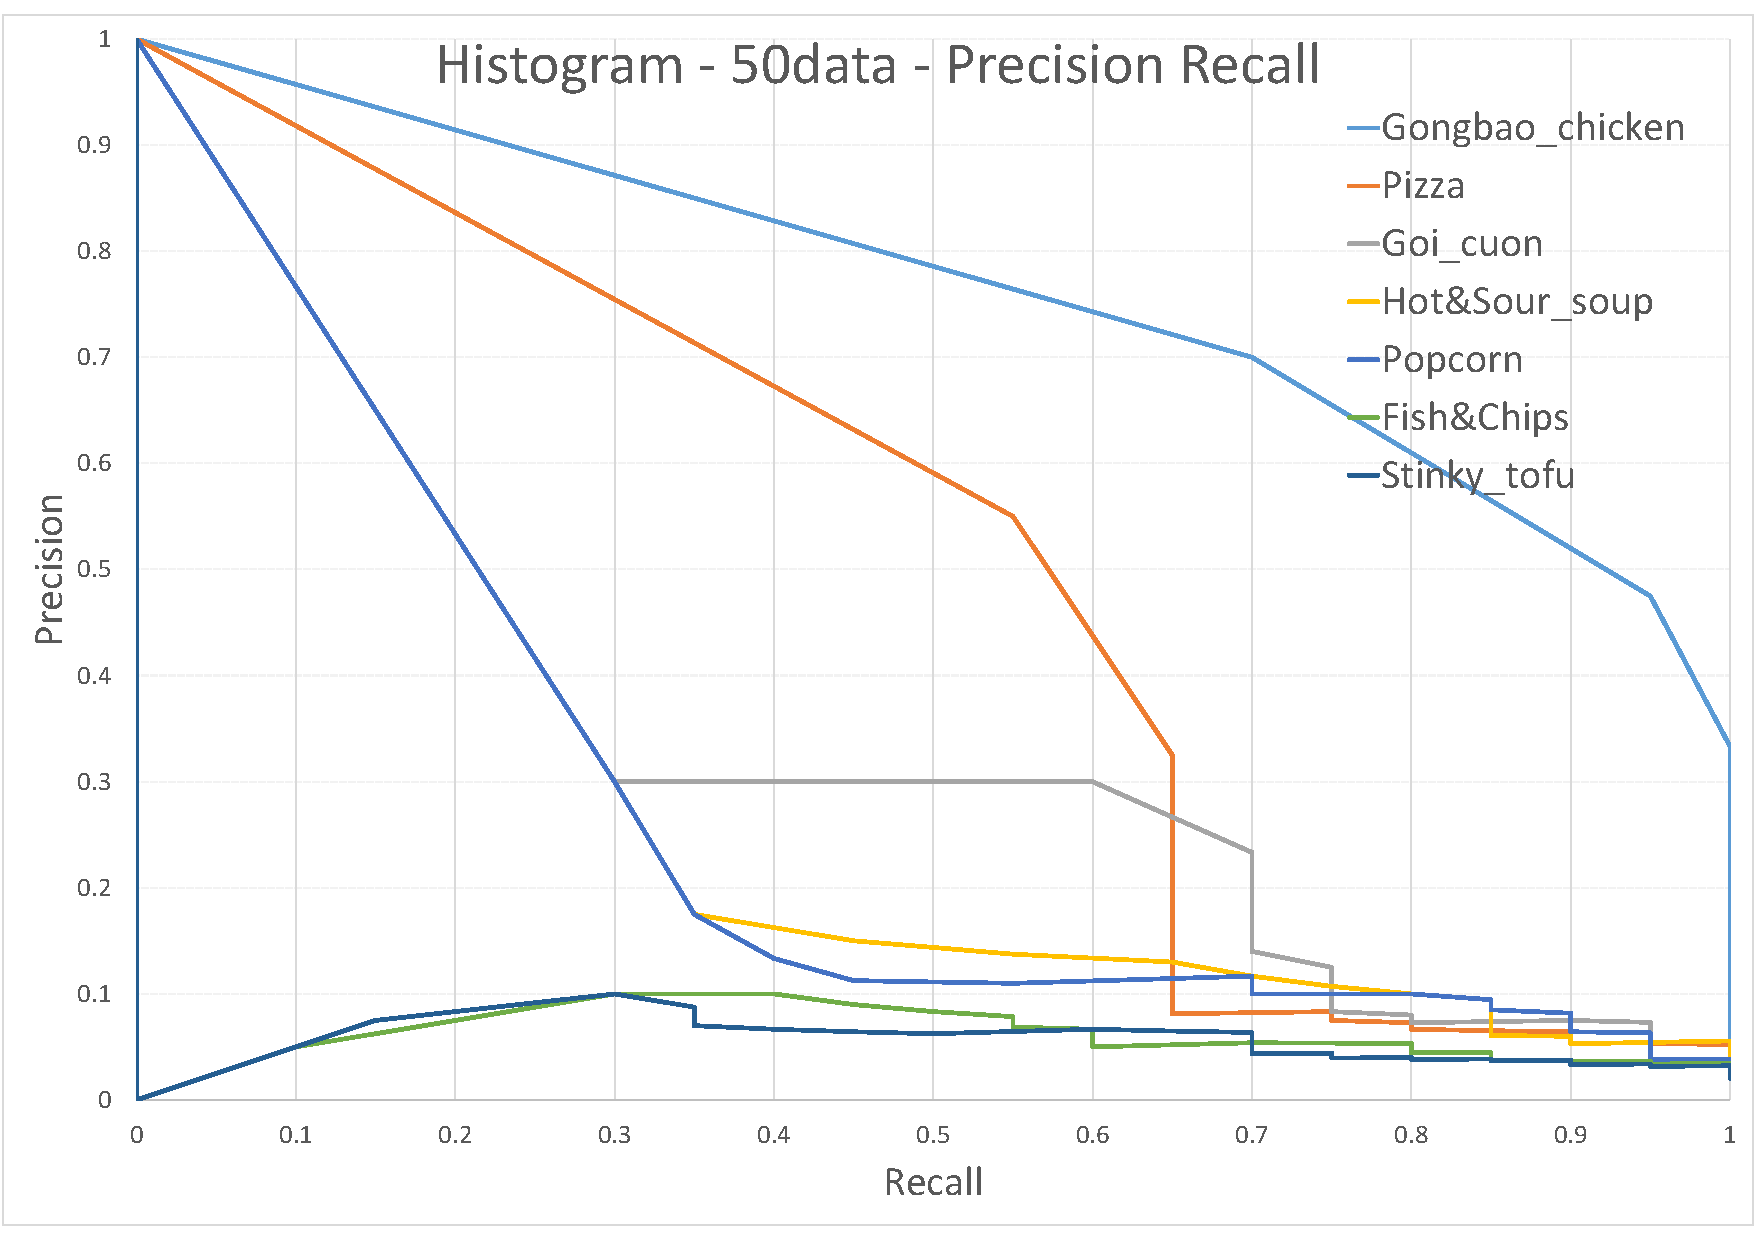
\includegraphics[width=75mm]{figures/results_HIST_50data_roc}}
	\subfloat[ORB]{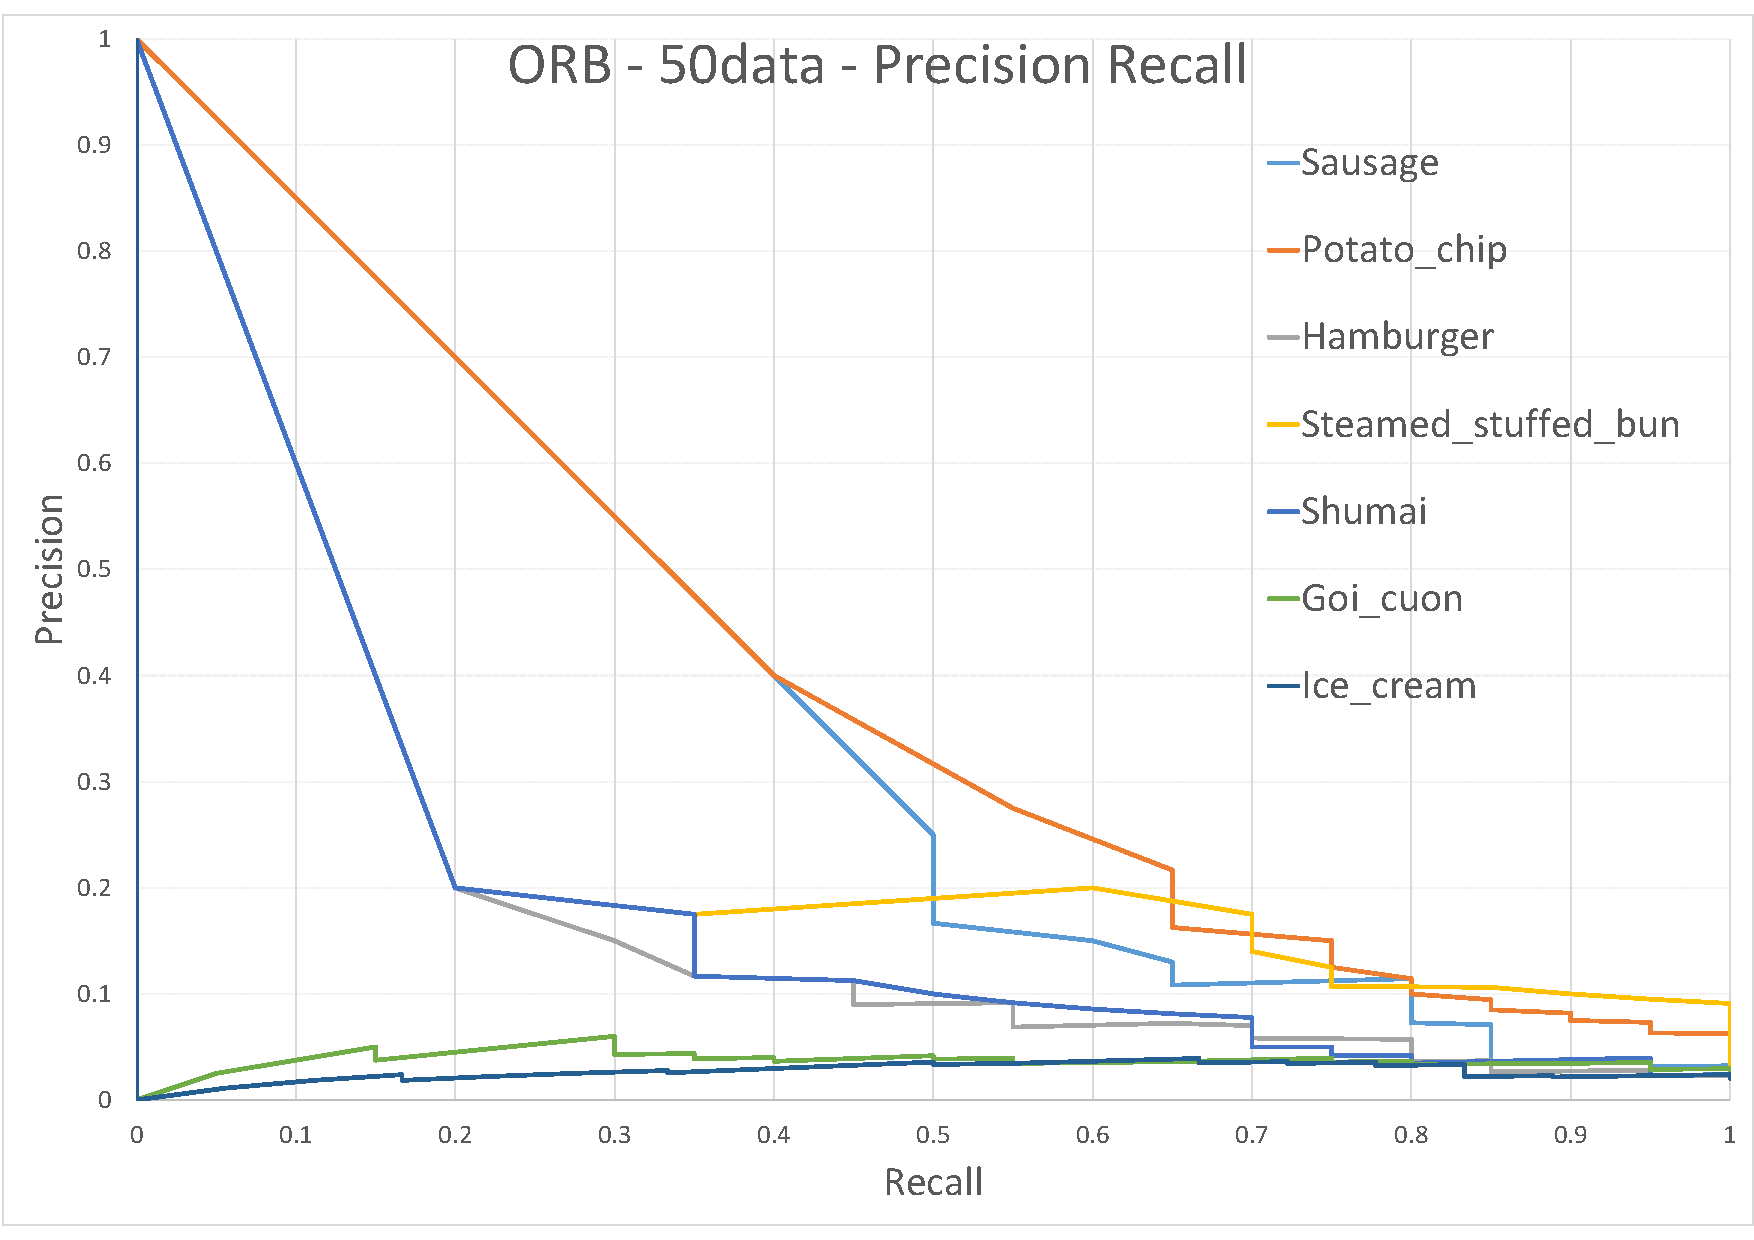
\includegraphics[width=75mm]{figures/results_ORB_50data_roc}}
	\caption{Precision recall curve for color histograms and ORB on the 50-data dataset validation segment.}
	\label{fig:results_HISTORBroc}
\end{figure}

On the full 50-data dataset the histogram classifier achieved an average top-1 validation accuracy of 0.2931. This is 14.7 times better than the null score. The standard deviation of the validation accuracy across all 50 classes is 0.151.

Figure \ref{fig:results_HISTORBroc}a shows the precision recall curve for the two best and worst classes as well as 3 classes around the median of the Top-1 validation accuracy. Figure \ref{fig:results_conv}f shows the confusion matrix for the histogram evaluation.

The histogram classifier had the most problems with "fish and chips" and "stinky tofu". The color of the class "Fish and chips" is very similar to the class "fried food" and "fish and chips" gets often confused with "fried food".
The two classes with the highest accuracy are "pizza" and "gongbao chicken".

\subsubsection*{Food-10}

The computational cost for the training of color histograms is very low. Therefore, this classifier was also tested on the much larger Food-100 dataset. The classifier was tested using 5-fold cross validation and achieved an average Top-1 accuracy on the validation set of 0.1758 with a maximum accuracy of 0.185.

\subsection{ORB}

\gls{orb} was tested with 1088 keypoints per image with both keypoint filtering and random point sampling turned on. A \gls{bow} with a vocabulary size of 2000 bins was used and images were loaded with a size of 262,144 pixels. For classification, a $\chi^2$ \gls{svm} was utilized.

The model achieved an accuracy of 0.2011 with a standard deviation over the accuracy of 0.1027. The accuracy is only half as good as \gls{surf} features. Nonetheless, this is still a better result than expected. \gls{orb} uses \gls{brief} as a descriptor which is a binary-test descriptor but the clustering used for the vocabulary creation by the OpenCV library is only indented to be used with floating point descriptors. So the descriptor clustering is not optimal for an \gls{orb} classifier which explains the poor performance.

Figure \ref{fig:results_HISTORBroc}b shows the precision recall curve for \gls{orb}. "Sausages" and "Potato chips" achieved the highest accuracies and "Goi cuon" and "ice cream" achieved the lowest accuracies.

\subsection{LBP}
\gls{lbp} achieved an accuracy of 0.119 which is only barely better than the null score. This is probably due to the fact that the basic LBP is a texture classifier and only contrast and illumination invariant. For food, however, rotation invariance is very important since food has no dominant orientation and plates can be freely rotated.
\subsection{CenSurE}
\gls{censure} was trained on images with the size 262,144 with the keypoint filtering turned off because the \gls{censure} \gls{api} of skimage does not provide a keypoint response so the score can not be calculated. SURF was used as the keypoint descriptor. Therefore, the number of extracted keypoints and the size of the bag of words vocabulary are the same. Since this is also a classifier with a \gls{bow}, the $\chi^2$ SVM kernel was used. The training of \gls{censure} took almost 33 hours and the top-1 accuracy is not very good. The top-5 accuracy, however, is very good and is actually the second best performance.

\subsection{Neural Network}
Three convolutional neural network architectures were used for evaluation. The first one is a deep \gls{cnn} with 15 layers:
\newline \newline
\begin{tabular}{lll}
	\textbf{Input} & $3 \times 48 \times 48$ &  \\ 
	\textbf{Convolutional Layer} & $32 \times 46 \times 46$ & $5 \times 5$ filters\\ 
	\textbf{Max Pooling Layer} & $32 \times 23 \times 23$ & $2 \times 2$ pooling\\ 
	\textbf{Dropout} & & 0.3\\ 
	
	\textbf{Convolutional Layer} & $64 \times 21 \times 21$ & $5 \times 5$ filters\\ 
	\textbf{Max Pooling Layer} & $64 \times 10 \times 10$ & $2 \times 2$ pooling\\ 
	\textbf{Dropout} & & 0.5\\ 
	
	\textbf{Convolutional Layer} & $128 \times 8 \times 8$ & $3 \times 3$ filters\\ 
	\textbf{Max Pooling Layer} & $128 \times 4 \times 4$ & $2 \times 2$ pooling\\ 
	\textbf{Dropout} & & 0.6\\ 
	
	\textbf{Dense Layer} & $512$ & \\ 
	\textbf{Dropout} & & 0.7\\ 
	\textbf{Dense Layer} & $512$ & \\ 
	\textbf{Dropout} & & 0.7\\ 
	
	\textbf{Output Layer} & 6 & \\ 
\end{tabular} 
\newline\newline
On 6 food classes this architecture achieved an accuracy of 0.2487 after 375 epochs and 7.5 hours of training.

The second network is a very small and compact 8-layer convolutional network: 
\newline \newline
\begin{tabular}{lll}
	\textbf{Input} & $3 \times 32 \times 32$ &  \\ 
	\textbf{Convolutional Layer} & $20 \times 32 \times 32$ & $5 \times 5$ filters\\ 
	\textbf{Max Pooling Layer} & $20 \times 16 \times 16$ & $2 \times 2$ pooling\\ 
	
	\textbf{Convolutional Layer} & $20 \times 16 \times 16$ & $5 \times 5$ filters\\ 
	\textbf{Max Pooling Layer} & $20 \times 8 \times 8$ & $2 \times 2$ pooling\\ 
	\textbf{Dropout} & & 0.5\\ 	
	
	\textbf{Dense Layer} & $1000$ & \\ 	
	\textbf{Output Layer} & 8 & \\ 
\end{tabular} 
\newline \newline
The advantage of this network is the fast training time and the ability to train it on smaller datasets. The network was trained on a 8 class subsample of the 50-data dataset and achieved a Top-1 accuracy of 0.4857 after 1912 epochs of training.

\section{Results for Size Estimation}

The image segmentation and size estimation modules are simple proof of concepts and were therefore only tested on images of menus from the canteen in Garching for the multi food item segmentation as well as home cooked, single type meals for the meal segmentation. All images were taken using a 41 mega pixel smartphone camera and were resized to fit a resolution of $1000 \times 564$.

\subsection{Single Meal Segmentation and Size Estimation}
\begin{figure}[htb]
	\centering
	\hspace{\fill}%
	\subfloat[canteen menu 1]{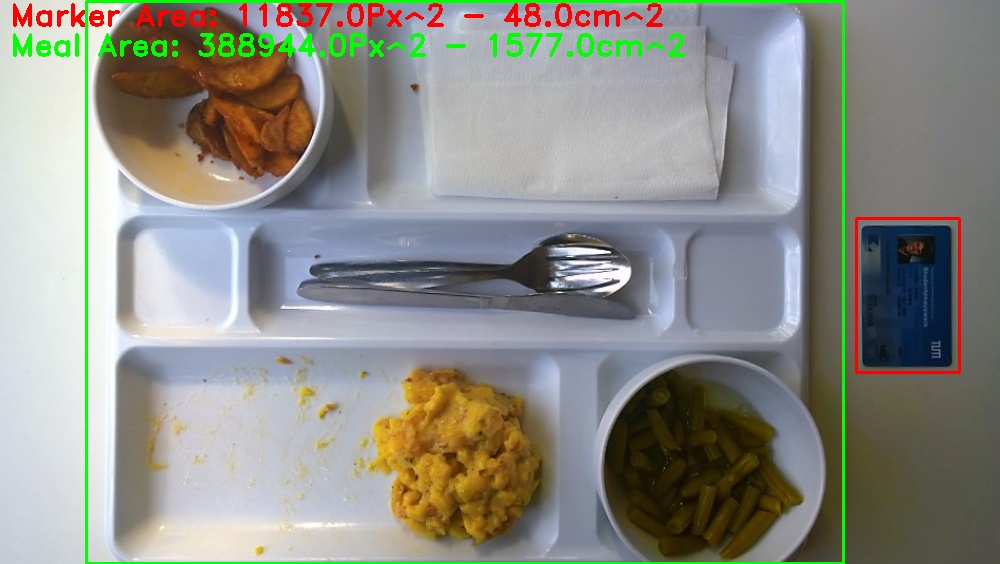
\includegraphics[height=18mm]{data/images/results/segmentation/resultsMarker_4_regions}}
	\hspace{\fill}%
	\subfloat[canteen menu 2]{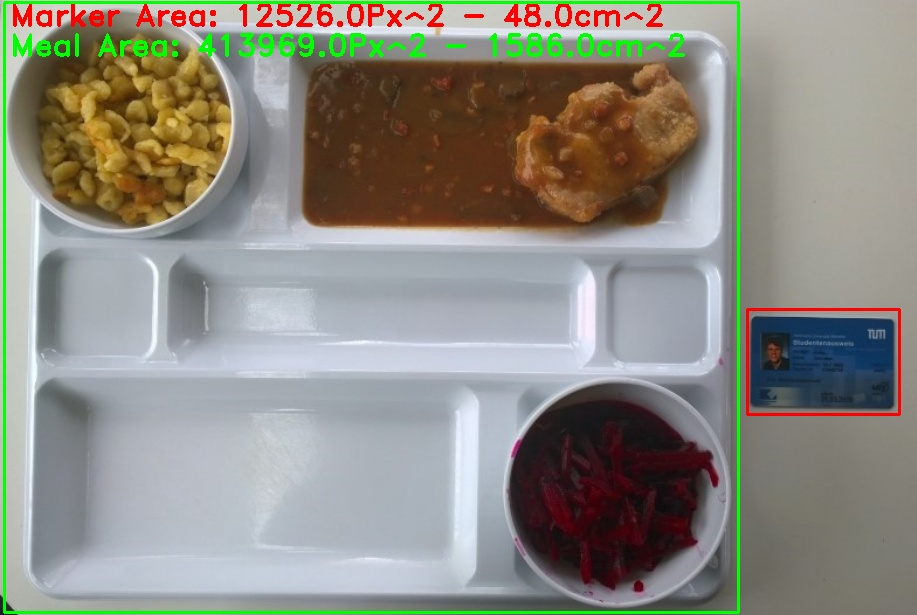
\includegraphics[height=18mm]{data/images/results/segmentation/resultsMarker_5_regions}}
	\hspace{\fill}%
	\subfloat[single food 1]{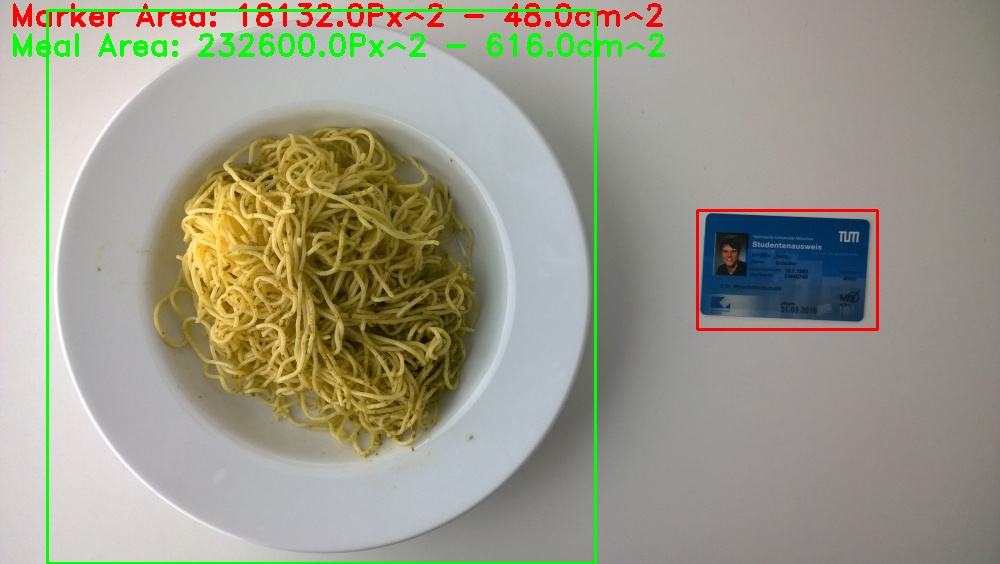
\includegraphics[height=18mm]{data/images/results/segmentation/resultsMarker_3_regions}}
	\hspace{\fill}%
	\subfloat[single food 2]{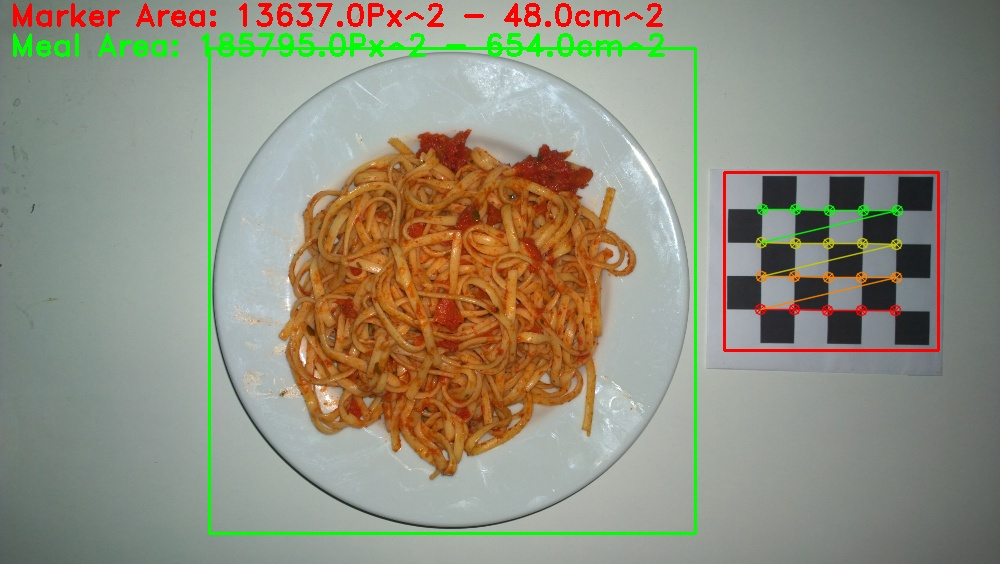
\includegraphics[height=18mm]{data/images/results/segmentation/resultsMarker_6_regions}}
	\hspace{\fill}%
	\caption{Meal region segmentation and size estimation. Calculated meal sizes: {(a)} $1577 cm^2$, {(b)} $1586 cm^2$, {(c)} $616 cm^2$, {(d)} $654 cm^2$}
	\label{fig:mealSegmentation}
\end{figure}

If the image of the food is taken from above with a clutter free and low contrast background the meal segmentation is reasonably fast and accurate. Almost all images were correctly segmented. Figure \ref{fig:mealSegmentation} shows 4 examples of the image segmentation with two canteen multi food menus measured with a custom marker and two single food images one with the custom marker and one with a chessboard marker. The difference between \ref{fig:mealSegmentation}a and \ref{fig:mealSegmentation}b is only $9 (cm)^2$ and $38 (cm)^2$ between the other two.

Marker recognition is not a problem either although there are issues with low contrast markers or markers that are too small or not rectangular. Due to SIFT's rotational invariance the recognition of rotated markers is still accurate. In figure \ref{fig:mealSegmentation}a the marker is rotated by 90\degree but the measurement and recognition is still accurate. Chessboard markers {(figure \ref{fig:mealSegmentation}d)} are even more accurate than arbitrary markers since they provide more fixed reference points.

\subsection{Multi Meal Segmentation and Size Estimation}
\begin{figure}[htb]
	\centering
	\hspace{\fill}%
	\subfloat[original image {(cropped)}]{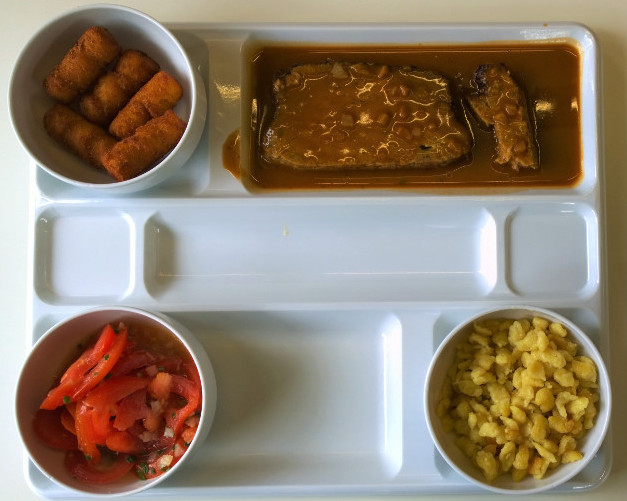
\includegraphics[height=20mm]{data/images/results/segmentation/results_1_original}}
	\hspace{\fill}%
	\subfloat[filtered image]{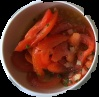
\includegraphics[height=20mm]{data/images/results/segmentation/resultsMarker_1_regionsArea-2}}
	\hspace{\fill}%
	\subfloat[filtered image]{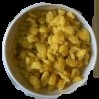
\includegraphics[height=20mm]{data/images/results/segmentation/resultsMarker_1_regionsArea-3}}
	\hspace{\fill}%
	\subfloat[filtered image]{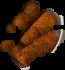
\includegraphics[height=20mm]{data/images/results/segmentation/resultsMarker_1_regionsArea-1}}
	\hspace{\fill}%
	\subfloat[filtered image]{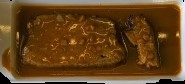
\includegraphics[height=20mm]{data/images/results/segmentation/resultsMarker_1_regionsArea-4}}
	\caption{Color filtering of 4 food items.}
	\label{fig:foodItemSegmentation}
\end{figure}
Although generally the concept of multi meal region segmentation works, this feature is still a work in progress and should be further developed in future works. Figure \ref{fig:foodItemSegmentation} shows images of the current state of the multi meal region segmentation. The problem here is, that dark or very bright colors are sometimes not correctly filtered. In addition there are issues with overlapping bounding boxes that can cause objects to be recognized multiple times because if two colors are to similar to each other they filter the same object. 